\PassOptionsToPackage{unicode=true}{hyperref} % options for packages loaded elsewhere
\PassOptionsToPackage{hyphens}{url}
%
\documentclass[]{article}
\usepackage{lmodern}
\usepackage{amssymb,amsmath}
\usepackage{ifxetex,ifluatex}
\usepackage{fixltx2e} % provides \textsubscript
\ifnum 0\ifxetex 1\fi\ifluatex 1\fi=0 % if pdftex
  \usepackage[T1]{fontenc}
  \usepackage[utf8]{inputenc}
  \usepackage{textcomp} % provides euro and other symbols
\else % if luatex or xelatex
  \usepackage{unicode-math}
  \defaultfontfeatures{Ligatures=TeX,Scale=MatchLowercase}
\fi
% use upquote if available, for straight quotes in verbatim environments
\IfFileExists{upquote.sty}{\usepackage{upquote}}{}
% use microtype if available
\IfFileExists{microtype.sty}{%
\usepackage[]{microtype}
\UseMicrotypeSet[protrusion]{basicmath} % disable protrusion for tt fonts
}{}
\IfFileExists{parskip.sty}{%
\usepackage{parskip}
}{% else
\setlength{\parindent}{0pt}
\setlength{\parskip}{6pt plus 2pt minus 1pt}
}
\usepackage{hyperref}
\hypersetup{
            pdftitle={Phonotactic variation in Pama-Nyungan tree inference},
            pdfborder={0 0 0},
            breaklinks=true}
\urlstyle{same}  % don't use monospace font for urls
\usepackage[margin=1in]{geometry}
\usepackage{longtable,booktabs}
% Fix footnotes in tables (requires footnote package)
\IfFileExists{footnote.sty}{\usepackage{footnote}\makesavenoteenv{longtable}}{}
\usepackage{graphicx,grffile}
\makeatletter
\def\maxwidth{\ifdim\Gin@nat@width>\linewidth\linewidth\else\Gin@nat@width\fi}
\def\maxheight{\ifdim\Gin@nat@height>\textheight\textheight\else\Gin@nat@height\fi}
\makeatother
% Scale images if necessary, so that they will not overflow the page
% margins by default, and it is still possible to overwrite the defaults
% using explicit options in \includegraphics[width, height, ...]{}
\setkeys{Gin}{width=\maxwidth,height=\maxheight,keepaspectratio}
\setlength{\emergencystretch}{3em}  % prevent overfull lines
\providecommand{\tightlist}{%
  \setlength{\itemsep}{0pt}\setlength{\parskip}{0pt}}
\setcounter{secnumdepth}{5}
% Redefines (sub)paragraphs to behave more like sections
\ifx\paragraph\undefined\else
\let\oldparagraph\paragraph
\renewcommand{\paragraph}[1]{\oldparagraph{#1}\mbox{}}
\fi
\ifx\subparagraph\undefined\else
\let\oldsubparagraph\subparagraph
\renewcommand{\subparagraph}[1]{\oldsubparagraph{#1}\mbox{}}
\fi

% set default figure placement to htbp
\makeatletter
\def\fps@figure{htbp}
\makeatother

\usepackage{etoolbox}
\makeatletter
\providecommand{\subtitle}[1]{% add subtitle to \maketitle
  \apptocmd{\@title}{\par {\large #1 \par}}{}{}
}
\makeatother
\usepackage{booktabs}
\usepackage{longtable}
\usepackage{array}
\usepackage{multirow}
\usepackage{wrapfig}
\usepackage{float}
\usepackage{colortbl}
\usepackage{pdflscape}
\usepackage{tabu}
\usepackage{threeparttable}
\usepackage{threeparttablex}
\usepackage[normalem]{ulem}
\usepackage{makecell}
\usepackage{xcolor}
\usepackage[bibstyle=biblatex-sp-unified,citestyle=sp-authoryear-comp]{biblatex}
\addbibresource{references.bib}

\title{Phonotactic variation in Pama-Nyungan tree inference}
\author{}
\date{\vspace{-2.5em}}

\begin{document}
\maketitle

Summary: This paper evaluates whether phylogenetic tree inference in linguistics is strengthened by the inclusion of phonotactic information. We take \textasciitilde{}1400 binary phonotactic variables and several hundred frequency variables and combine them with lexical cognate data from 44 western Pama-Nyungan languages. The study begins with preliminary explores the evolutionary dynamics of the phonotactic data. This is necessary to ascertain the best evolutionary model with which to infer a tree, since this is a novel source of data in linguistic tree inference. The second part of the study compares two models for inferring a Pama-Nyungan phylogeny using Bayesian methods. In one, a phonotactic data partition and lexical cognate partition are used jointly to infer trees. In the other these partitions are kept separate for the purpose of tree inference. Bayes factors for these two models are compared. We find that the combination of phonotactic data with lexical data does not significantly strengthen tree inference, likely owing to deficiencies in the evolutionary model and current computational limitiations. The paper concludes with a discussion of the reasons for this and an outline of future research steps to evaluate whether the present findings represent a true negative or merely limitations of the methodology.

\textbf{Notes:}

Bayes factors are robust \autocite{brown_importance_2007}

\hypertarget{pn-tree-intro}{%
\section{Introduction}\label{pn-tree-intro}}

\emph{This section needs fleshing out, but not too much. Aim is to keep it sharp and concise}.

Background:

Phylogenies in linguistics are a big deal.

Lots of tree building been happening.

Phylogenies are also crucial for advances in comparative langauge sciences, studies of human history generally.

Data mainly limited to cognates. Some use of structural characters, but these tend to suffer from restricted state space.

In biology, \textcite{parins-fukuchi_use_2018} find that combining continuous morphological characters to more traditional, categorical data can strengthen tree inference. An example of integration of continuous morphological data and genomic data \textcite{domel_combining_2019}.

Prev. study \autocite{macklin-cordes_phylogenetic_2020} found phylogenetic signal in phonotactics. The hypothesis was that phonotactic systems are likely to evolve in an historically conservative way, reflect linguistic phylogenies and therefore be useful for tree inference. That finding was encouraging support for this hypothesis but not definitive proof by any means. Just because something has phylogenetic signal does not mean, by itself, that you can infer phylogenetic trees from it. For example, geography often has a pretty strong phylogenetic signal. In this study, we put the hypothesis to the test by attempting to infer a linguistic phylogeny with the aid of phonotactics.

\hypertarget{why-phonotactics}{%
\subsection{Why phonotactics}\label{why-phonotactics}}

\textbf{revise}

We are motivated to extract frequency datasets for a couple of reasons. Firstly, it allows us to capture a finer grained level of information than binary data would allow. Binary data is more similar to the kind of phonotactic information one might find in a published language grammar, where a description of phonotactics that one would typically encounter involves a series of statements on the (binary) permissibility or otherwise of certain combination of segments. This information does not, however, account for quantitative differences between common, high frequency sequences of segments versus dispreferred sequences that rarely arise in a language's lexicon. There is considerable evidence to suggest that speakers are psychologically attuned to these kinds of phonological frequencies \autocites{coleman_stochastic_1997}{zuraw_patterned_2000}{ernestus_predicting_2003}{albright_rules_2003}{eddington_spanish_2004}{hayes_stochastic_2006}{gordon_phonological_2016}. The second reason is that the relatively rapid, semi-automated extraction of transition frequencies from wordlists captures structural variation between languages at a scale and degree of precision that would be difficult to attain from manual data coding methods (as preferred for the coding of lexical cognate data and grammatical data used in previous linguistic phylogenetic work). \textcite{macklin-cordes_phylogenetic_2020} show that this transition frequency dataset contains stronger phylogenetic signal than its binary equivalent. There is one limitation of the frequency transition data, which is that presently we require positive values to use for tree inference (more on evolutionary models and tree inference below). Biphones of zero frequency (recorded as `0' in the binary dataset) get transformed to gaps in the dataset. By including the binary dataset in this study, we retain a distinction between biphones that are impossible in a language (because one or both of the segments are absent from the language's phonemic inventory) and biphones that are possible in principle but are never observed. Our phonotactic data captures information on which phonemic segments may combine immediately adjacent to one another and the frequencies at which they do so. This is phonotactics in the simplest sense, and does not directly capture phonotactic restrictions that depend on sequences beyond two segments, syllable structure or morpheme boundaries. Nevertheless, \textcite{macklin-cordes_phylogenetic_2020} confirm that this simple level of phonotactic data is sufficieent to detect strong phylogenetic signal.

Another argument is that our method avoids \emph{observer bias}. We don't have to rely on an expert picking and choosing which parts of a grammatical or lexical system are interesting and worth coding. This is described as an advantage of large-scale extraction of continuous morphological characters in biology too \autocite{wright_systematists_2019}. Another advantage of encoding structural variation with continuous characters over categorical ones: ``phylogenetic error is very high for characters with \ldots{} very high rates of evolution (due to homoplasy of changes). Continuous characters do not display this relationship as strongly due to their large state space, though more research is needed to demonstrate this effect empirically.'' \autocite{wright_bayesian_2014}. Applicable to grammatical variables in linguistic phylogenetic tree inference, which show high rates of evolution and lots of homoplasy, due at least in part to tightly contrained state space \autocite{greenhill_evolutionary_2017}. We don't have to worry about correcting for acquisition bias since the datasets reflect the full range of logically possible biphones in every language. We can include invariant sites (where all values are the same. These don't matter much for topology but are important for dating/branch lengths) and we don't need to correct for ascertainment bias \autocite{leache_short_2015}.

We use a Bayesian computational approach to infer linguistic phylogenies using BEAST phylogenetic software (v1.10.5) \autocite{suchard_bayesian_2018}. This is similar to earlier work on the Pama-Nyungan phylogeny \autocites{bowern_computational_2012}{bouckaert_origin_2018} which used BEAST2 \autocite{bouckaert_beast_2019}. We selected BEAST over BEAST2 because it offers the ability to infer trees with continuous characters. Throughout, we generally try to follow \textcite{bouckaert_origin_2018} as closely as possible. We follow \textcite{bouckaert_origin_2018} in constraining the tree topology using clade priors for well-established and commonly accepted Pama-Nyungan subgroups, as established by \textcite{ogrady_languages_1966}, \textcite{muhlhausler_atlas_1996} and \textcite{koch_languages_2014} and subsequently recovered in computational phylogenetic analysis by \textcite{bowern_computational_2012}. Dating the Pama-Nyungan tree is a central focus of \textcite{bouckaert_origin_2018}, combining lexical cognate data with geographical data and archaeological calibration points to give a best-available estimate of the geographic and temporal point of origin of the family. Accordingly, we retain their calibration prior on the Wati subgroup, which places a 95\% probability of the subgroup's origin dating between 3,000-5,000 years, with most of the probability density skewing towards the younger end of that range (a gamma distribution of \(\alpha = 2\), \(\beta = 359\), with 3,000 year offset) based on a synthesis of archaeological evidence \autocite[see][p.~746]{bouckaert_origin_2018}. We place a prior on the root age of the Pama-Nyungan family centred on a mean of 5,791 years B.P., following the findings of \textcite{bouckaert_origin_2018}. 5,791 years is the mean root age of the posterior for their best supported hypothesis on Pama-Nyungan's origins. We model this as a normal distribution (SD = 730) approximating the 95\% range of posterior root age estimates. One aspect in which we differ from \textcite{bouckaert_origin_2018} is tip dates. \textcite{bouckaert_origin_2018} use a birth-death skyline tree model which allows for tip dates to differ and includes a parameter corresponding to the proportion of total taxa sampled at a given point in time. This is reasonable since they use language sources span over 200 years. In contrast, we assume all tips are contemporaneous. In our case, since we restrict attention to relatively modern sources, any extra precision to be gained from including tip dates is not worth the reduced tree model choice in BEAST and extra computational expence.

\hypertarget{pn-tree-combined}{%
\subsection{Combined cognate and phonotactics tree inference}\label{pn-tree-combined}}

Evolutionary model for phonotactic frequency dataset is more straightforward. We take a standard, lightweight Brownian motion model in which frequency values can wander up or down with equal probability through time. We are limited to this model by software constraints, but that is not a major limitation at this point. Firstly, Brownian motion is a standard starting point in comparable biological studies that jointly infer trees with continuous data. Secondly, it is the same model used in \textcite{macklin-cordes_phylogenetic_2020}. One difference between \textcite{macklin-cordes_phylogenetic_2020} and this study is that \textcite{macklin-cordes_phylogenetic_2020} use raw frequency values whereas we use log-transformed frequency values. We observe that biphone transition frequencies tend to be skewed such that lexicons tend to contain relatively few high frequency biphone transitions and many low frequency transitions. It follows then that these biphone transition frequencies are more likely the outcome of an evolutionary process where characters wander along a skewed, lognormal scale than one in which they wander along a normal distribution (although, in practice, it may not matter too much. \textcite{macklin-cordes_phylogenetic_2020} find no significant difference in phylogenetic signal using raw values versus log-transformed values). These skewed distributions echo the skewed distributions of single segments observed by \textcite{macklin-cordes_re-evaluating_2020}. As \textcite{macklin-cordes_re-evaluating_2020} makes clear, this does not mean that biphone transition frequencies are necessarily drawn from a lognormal distribution and a more sophisticated maximum likelihood test would be needed to distinguish between the lognormal and several other similarly skewed distribution types. Nevertheless, the lognormal distribution is a sufficient approximation of the skewed distribution of biphone transition frequencies for our purposes in this study.

Thinking briefly about what would be a realistic model of evolution for biphone transition frequencies. We would expect there to be two main forces impacting these frequencies. The first is the introduction of new vocabulary to a language via lexical innovation or borrowing. Each new word entering a lexicon will alter minutely the frequencies of biphone transitions in the language (similarly, transition frequencies will decline as words are replaced or fall out of usage). This is the kind of gradual accumulation of changes that we might expect to follow a Brownian motion-like pattern of evolution (although maybe the rates of going up and down are not equal). Further, since speakers show a preference for high frequency phonotactic sequences over low frequency sequences when coining new words, we might expect this accumulation of changes to follow a kind of `rich get richer' process which would result in the kind of skewed frequency distributions that we observe. Also, when languages borrow vocabulary, the trend is for foreign words with dispreferred phonotactic sequences to shift towards more natively preferred patterns (sometimes gradually over a long period of time, i.e.~look at various French words in English, stress has shifted to English pattern in some but not yet in others), which would strengthen this kind of `rich get richer' process and also keep phonotactic frequency data historically conservative. The second major force on biphone frequencies is sound change. We would expect sound changes to result in sudden jumps in the frequencies of affected biphones, sometimes to 0 or 1. Our binary characters capture some of these effects to a limited extent. For example, perhaps a language has some frequency value for sequences of a nasal followed by a stop with a different place of articulation. If that nasal undergoes place assimilation, the biphone frequency will drop to 0 and thus disappears as a gap in the frequency dataset since evolutionary model requires non-zero values. On the other hand, this assimilation will be recorded in the binary data as a shift from `1' to `0'. In other instances, biphone characters may shift from missing to present and vice versa in both the frequency and binary datasets. For example, if a contrastive vowel length distinction emerges, certain biphones (namely those with long vowels) will go from being a gap in a language's biphone transition frequency data to some positive, non-missing value. In the case of a merger between short and long vowels, the opposite will be true. Our model, at present, simply does not account well for sound change. In this respect, there is an advantage to studying Australian languages, since Australian languages show uniquely constrained variation in phonological inventories {[}REFS{]} (easier to match biphones between languages, less dataset sparsity) and less history of identified sound changes relative to other parts of the world (historical linguists have long turned to sources of historical evidence in other parts of language like morphology etc. {[}REFS{]}). We return to this subject in Section \ref{pn-tree-discussion}.

For the cognate data partition, we approximate as much as possible the best supported priors from \textcite{bouckaert_origin_2018}. We use a covarion model with a relaxed clock and fixed rates across cognate classes.

\hypertarget{methodology}{%
\section{Methodology}\label{methodology}}

\hypertarget{research-question}{%
\subsection{Research question}\label{research-question}}

This study tests the question of whether or not the addition of phonotactic data strengthens linguistic phylogenetic tree inference. To test this question, we infer a phylogeny of the western branch of Pama-Nyungan languages using lexical cognate data and phonotactic data and repeat this process twice---once in which the phylogeny is inferred jointly from cognate and phonotactic data and once in which separate trees are inferred from cognate data dand phonotactic data. The strength of phylogenetic inference in each instance is evaluated by estimating and comparing log marginal likelihoods for each, and comparing the topologies and posterior clade support values of maximum clade credibility trees.

\hypertarget{experimental-design}{%
\subsection{Experimental design}\label{experimental-design}}

There are four test components in this study: two preliminary test components and two main test components. Preliminary testing consists of (1) evaluating the best-fitting evolutionary model for binary biphone data, and (2) tree inference using cognate data only, essentially aiming to replicate \textcite{bouckaert_origin_2018}. Model comparison is a regular step in linguistic phylogenetic studies, as typically a number of clock models, site models and other parameters are considered. In this study, the cognate data is sourced from a prior study \autocite{bouckaert_origin_2018} which already evaluated the best-fitting model for this particular set of data. Accordingly, we skip this process and replicate as much as possible the best supported model and priors that \textcite{bouckaert_origin_2018} find. It is a different story, however, for the binary biphone data which has not been used previously for phylogenetic tree inference. The novelty of this data source necessitates a thorough evaluation of which evolutionary model can best be applied to it. This is the subject of the first preliminary test.

The second preliminary test involves inferring a phylogeny using only cognate data from \textcite{bouckaert_origin_2018}. This test functions as a sanity check to ensure that our phylogenetic model and software implementation, which approximates but does not exactly replicate \textcite{bouckaert_origin_2018}, produces suitably equivalent results.

These preliminary tests are followed by the main test evaluating the primary research question described above. We use the Bayesian Markov chain Monte Carlo (MCMC) method implemented in BEAST phylogenetic software to infer a phylogeny of western Pama-Nyungan using cognate data, binary biphone data and continuous phonotactic data consisting of sound class transition frequencies. In a second MCMC run, we include two tree models, one inferred with cognate data only and another with phonotactic data only (both binary and continuous). Marginal likelihoods are estimated using the stepping stone sampling method \autocite{baele_accurate_2013}. For each tree model, we produce a maximum clade credibility tree from the posterior sample of trees that BEAST produces and then compare the topologies and clade support values of these.

We conduct one follow-up test after this. To test our suspicion that the binary phonotactic data was contributing undue weight to likelihood calculations without contributing much phylogenetic information, we re-ran the experiment with this data partition removed. In this instance, the second BEAST run contains two tree models, one inferred with cognate data only and one inferred using cognate data and continuous phonotactic data together.

\hypertarget{language-sample}{%
\subsection{Language sample}\label{language-sample}}

The target language sample, in the first instance, is the 306 Pama-Nyungan language varieties represented in \textcite{bouckaert_origin_2018}. Of these, we restrict attention to languages meeting the following criteria. Firstly, the language must be represented in the Ausphon Lexicon database \autocite[@][]{round_ausphon-lexicon_2017} from which we source wordlist data. Secondly, the original wordlist data source must have been compiled by a trained linguist from primary fieldwork with living speakers or a combination of fieldwork and archival materials (no sources reconstituted only from archival materials). Thirdly, each wordlist must contain at least 250 lexical items. This leaves a subset of 111 Pama-Nyungan languages. In Preliminary Test 1, where computational demands are relatively minimal, this is the language sample we use. Due to computational constraints associated with large amounts of continuous data and large phylogenies, in the main test we restrict attention to the western branch of the Pama-Nyungan family identified in \textcite{bowern_computational_2012} and \textcite{bouckaert_origin_2018}. This gives a sample of 44 western Pama-Nyungan languages covering nine Pama-Nyungan subgroups. A list of languages and their original sources is available in \textbf{APPENDIX REF}.

\hypertarget{prelim-1}{%
\section{Preliminary test 1: Evolutionary model for binary biphone data}\label{prelim-1}}

As the number of linguistic phylogenetic studies using lexical cognate data expands, some consistent findings have emerged, for example covarion model seems widely preferred. {[}check state of the art language comparison article{]}. However, this is to the best of our knowledge the first attempt at tree inference with binary biphone characters {[}unless Gerhart tried it?{]} so we start by embarking on the process of model testing and selection for this novel data type. The aim is to identify a sensible model and set of priors that we can specify for the binary biphone data in subsequent testing.

For each model specification, we run two independent MCMC chains of 25,000,000 iterations, with parameters logged every 10,000 iterations. Log marginal likelihoods are estimated using BEAST's path sampling/stepping stone sampling procedure \autocites{baele_improving_2012}{baele_accurate_2013} consisting of 50 path steps of 500,000 iterations, with parameters logged every 10,000 iterations, conducted on each chain then combined to get an overall marginal likelihood estimate (MLE). We conducted autocorrelation and convergence checks using Tracer v1.7.1 software \autocite{rambaut_posterior_2018}. Note that the results here are a preliminary exploration of model parameters to determine the best parameter settings for the tree inference presented in Section \ref{pn-tree-combined} below. We do not anticipate that binary biphone characters will produce especially high quality or realistic language phylogenies on their own. The goal is to get a handle on how best to model the evolutionary dynamics of this dataset when used in combination with other sources of evidence.

We test a total of 16 models, consisting of each logically possible combination of site and clock model components. We describe each of these alternatives in turn below.

\hypertarget{binary-biphone-data}{%
\subsection{Binary biphone data}\label{binary-biphone-data}}

A language's phonotactic system consists of rules governing how phonemic segments may combine into larger syllables and words. To represent phonotactics, we extract data on the presence and frequencies of \emph{biphones}, two-segment sequences, from language wordlists. From each wordlist, we extract data on the presence and absence of \emph{biphones}, sequences of two segments (where each segment is either a phoneme or a word boundary). A biphone is marked `1' if it is present anywhere in a language's wordlist. If the biphone consists of two segments that are part of the language's phonemic inventory (and therefore the biphone could, in principle, occur in the language) but the biphone never occurs, it is marked `0' for absent. If one or both segments in the biphone are not part of the language's phonemic inventory, then it is marked as a gap `-' in the data. A total of 2236 binary biphone characters are extracted.

\hypertarget{site-and-clock-settings}{%
\subsection{Site and clock settings}\label{site-and-clock-settings}}

Site models describe how binary biphone characters evolve through time. The site model is defined by three parameters, giving eight possible combinations to test:

For this stage of evaluation, we fix the clock model to a strict clock (no variation in evolutionary rates between branches) and fix the tree model to a simple calibrated Yule tree model with a uniform birth rate prior (Yule tree models do not allow for extinction events). We then test all eight combinations of three site model parameters:

\begin{itemize}
\tightlist
\item
  A simple continuous time Markov chain (CTMC) model (which contains a single estimated parameter that specifies the frequencies with which biphones are gained and lost) versus a covarion model (which allows sites to switch between fast and slow states). The covarion model is the preferred model of lexical cognate evolution in \textcite{bouckaert_corrections_2012}, \textcite{bouckaert_origin_2018} and \textcite{kolipakam_bayesian_2018}, although \textcite[p.~219]{chang_ancestry-constrained_2015} find little difference between them and opt for the increased simplicity of the former model.
\item
  Empirical character state frequencies versus estimated character state frequencies.
\item
  Site homogeneity (fixed evolutionary rates across all character sites) versus heterogeneity (estimated using four gamma distributed categories, following \textcite{kolipakam_bayesian_2018}). For cognate data, \textcite{bouckaert_origin_2018} find a better fit with homgenous rates but \textcite{kolipakam_bayesian_2018} find a better fit with heterogenous ones.
\end{itemize}

We use Bayes factors to determine the best supported site, clock and tree models. Bayes factors give an indication of the support for one model over another and are calculated by calculating the ratio of the log marginal likelihoods of each model. A Bayes factor of 5 to 20 is taken as substantial support, greater than 20 as strong support, and greater than 100 as decisive \autocite{kass_bayes_1995}. We table Bayes factors comparing each combination of model settings in Table \ref{tab:site-models}. The names of each model indicate site settings as follows: (S)imple CTMC versus (C)ovarion model, e(M)pirical versus e(S)timated character frequencies, (H)omogenous rates versus (G)amma-distributed heterogenous rates. So, for example, the model termed ``CMH'' consists of a covarion model with empirical frequencies and homogenous rates across all sites.

We test two clock models: A strict clock, in which a single evolutionary rate is fixed across all branches in the tree, and a lognormally-distributed, uncorrelated relaxed clock. This relaxed clock model generally has been found to outperform a strict clock when modelling lexical cognate evolution \autocites{bouckaert_origin_2018}{kolipakam_bayesian_2018}. Clock settings are denoted in Table \ref{tab:site-models} by `S' for strict and `R' for relaxed. So, for example, the model termed ``SSG-S'' is a simple site model with estimated character frequencies and gamma-distributed heterogenous rates, combined with a strict clock.

For the relaxed clock, we used an uncorrelated lognormal setting with a uniform prior {[}0,1{]} following \textcite{kolipakam_bayesian_2018}. \textcite{bouckaert_origin_2018} constrain the upper bound to 1.0E-4 to reduce burn-in time since, in practice, the mean clock value never approaches even that level. We chose the less informative upper bound given the uncertainty of working with a novel data type.

A third Bayesian phylogenetic model component is the tree model which defines the speciation process. Two main alternatives appear frequently in linguistic phylogenetic research. These are birth-death speciation models, which allow for extinction events, and Yule speciation models, which allow birth events only \autocites[as preferred in][]{bowern_computational_2012}{kolipakam_bayesian_2018}. \textcite{bouckaert_origin_2018} use a Birth-Death Skyline model which enables tips to be sampled at different dates, but fix the death rate to zero. This is reasonable since they use language sources span over 200 years. Throughout this study, we follow this precedent by using a birth-death model with the death rate set to zero. However, instead of including different tip ages, we assume all tips are contemporaneous and set their ages to 0, which is not strictly accurate since original wordlist sources do vary in age. In our case, since we restrict attention to relatively modern sources, any extra precision to be gained from including tip dates is not worth the reduced tree model choice in BEAST and extra computational expense. One additional parameter that we do include instead is an incomplete sampling parameter to account for the fact that our language sample is only a subset of the full 306 languages included in \textcite{bouckaert_origin_2018}. this incomplete sampling parameter is set to 0.36 in this preliminary test (\(\frac{111}{306}\)).

\hypertarget{results-prelim-1}{%
\subsection{Results}\label{results-prelim-1}}

Bayes factors of pairwise comparisons between candidate models are listed in Table \ref{tab:site-models}. The covarion model overwhelmingly outperforms the simple CTMC model in all instances. Furthermore, there is support for allowing evolutionary rates to vary across character sites. Unfortunately, this great increase in parameters results in a corresponding increase in computational demand. Models with heterogenous rates require 3--4 times as long as equivalent models with fixed rates. Secondly, there is decisive support for estimating character state frequencies rather than simply taking the observed frequencies when the covarion model is used, although the opposite is true with a CTMC model. A covarion model with estimated frequencies and homogenous evolutionary rates will score higher than a model where rates are allowed to vary but empirical frequencies are used. All up, we determine the best site model to be a covarion model with estimated frequencies and rate heterogeneity.

With regards to the clock model, site models paired with a relaxed clock tend to do better than their direct equivalents paired with a strict clock, though covarion models with homogenous rates are exceptions. The best site model, denoted `CSG' (covarion, estimated frequencies, gamma heterogenous rates), scores decisively higher than all others regardless of which clock model is used. The `winning' model, which we proceed to apply to binary biphone data throughout the rest of this study, is the CSG model with a relaxed clock (`CSG-R').

\begin{landscape}\begin{table}

\caption{\label{tab:site-models}Bayes factors for different site models. Each Bayes Factor represents the support for one model (vertical axis) against another (horizontal). A positive value indicates the first model (left) is supported, and conversely, a negative value indicates the second model (top) is supported. A value over 100 is considered decisive.}
\centering
\fontsize{8}{10}\selectfont
\begin{tabular}[t]{lrrrrrrrrrrrrrrrr}
\toprule
Site model & CMG-R & CMG-S & CMH-R & CMH-S & CSG-R & CSG-S & CSH-R & CSH-S & SMG-R & SMG-S & SMH-R & SMH-S & SSG-R & SSG-S & SSH-R & SSH-S\\
\midrule
CMG-R & -- & 20,274 & 44,531 & 20,746 & -33,840 & -16,924 & 42,417 & 22,034 & 59,797 & 59,966 & 61,049 & 61,250 & 59,793 & 59,932 & 61,036 & 61,246\\
CMG-S & -20,274 & -- & 24,257 & 472 & -54,114 & -37,198 & 22,143 & 1,760 & 39,523 & 39,692 & 40,775 & 40,976 & 39,519 & 39,658 & 40,762 & 40,972\\
CMH-R & -44,531 & -24,257 & -- & -23,785 & -78,371 & -61,455 & -2,114 & -22,497 & 15,266 & 15,435 & 16,518 & 16,719 & 15,262 & 15,401 & 16,505 & 16,715\\
CMH-S & -20,746 & -472 & 23,785 & -- & -54,586 & -37,670 & 21,671 & 1,288 & 39,051 & 39,220 & 40,303 & 40,504 & 39,047 & 39,186 & 40,290 & 40,500\\
\addlinespace
CSG-R & 33,840 & 54,114 & 78,371 & 54,586 & -- & 16,916 & 76,257 & 55,874 & 93,637 & 93,806 & 94,889 & 95,090 & 93,633 & 93,772 & 94,876 & 95,086\\
CSG-S & 16,924 & 37,198 & 61,455 & 37,670 & -16,916 & -- & 59,341 & 38,958 & 76,721 & 76,890 & 77,973 & 78,174 & 76,717 & 76,856 & 77,960 & 78,170\\
CSH-R & -42,417 & -22,143 & 2,114 & -21,671 & -76,257 & -59,341 & -- & -20,383 & 17,380 & 17,549 & 18,632 & 18,833 & 17,376 & 17,515 & 18,619 & 18,829\\
CSH-S & -22,034 & -1,760 & 22,497 & -1,288 & -55,874 & -38,958 & 20,383 & -- & 37,763 & 37,932 & 39,015 & 39,216 & 37,759 & 37,898 & 39,002 & 39,212\\
\addlinespace
SMG-R & -59,797 & -39,523 & -15,266 & -39,051 & -93,637 & -76,721 & -17,380 & -37,763 & -- & 169 & 1,252 & 1,453 & -4 & 135 & 1,239 & 1,449\\
SMG-S & -59,966 & -39,692 & -15,435 & -39,220 & -93,806 & -76,890 & -17,549 & -37,932 & -169 & -- & 1,083 & 1,284 & -173 & -34 & 1,070 & 1,280\\
SMH-R & -61,049 & -40,775 & -16,518 & -40,303 & -94,889 & -77,973 & -18,632 & -39,015 & -1,252 & -1,083 & -- & 201 & -1,256 & -1,117 & -13 & 197\\
SMH-S & -61,250 & -40,976 & -16,719 & -40,504 & -95,090 & -78,174 & -18,833 & -39,216 & -1,453 & -1,284 & -201 & -- & -1,457 & -1,318 & -214 & -4\\
\addlinespace
SSG-R & -59,793 & -39,519 & -15,262 & -39,047 & -93,633 & -76,717 & -17,376 & -37,759 & 4 & 173 & 1,256 & 1,457 & -- & 139 & 1,243 & 1,453\\
SSG-S & -59,932 & -39,658 & -15,401 & -39,186 & -93,772 & -76,856 & -17,515 & -37,898 & -135 & 34 & 1,117 & 1,318 & -139 & -- & 1,104 & 1,314\\
SSH-R & -61,036 & -40,762 & -16,505 & -40,290 & -94,876 & -77,960 & -18,619 & -39,002 & -1,239 & -1,070 & 13 & 214 & -1,243 & -1,104 & -- & 210\\
SSH-S & -61,246 & -40,972 & -16,715 & -40,500 & -95,086 & -78,170 & -18,829 & -39,212 & -1,449 & -1,280 & -197 & 4 & -1,453 & -1,314 & -210 & --\\
\bottomrule
\end{tabular}
\end{table}
\end{landscape}

One limitation to note is that we have not considered the stochastic Dollo model, which has been implemented with some success for cognate data in linguistics \autocite{bowern_computational_2012} (although the covarion model was subsequently found to be better in \textcite{bouckaert_origin_2018}). Stochastic Dollo only allows characters to spring into existance once and any losses are permanent. Such a model is perhaps a bit more realistic for cognates, since the state space of possible words is practically infinite (i.e.~the chance of different people inventing the same word for the same thing independently is low, although of course it does happen sometimes)\footnote{That said, stochastic Dollo is not particularly realistic for cognates either since it does not allow for borrowing, which manifests as two independent origin points when plotted on a phylogenetic tree. The presence of borrowing likely explains why the covarion model tends to work better than stochastic Dollo in linguistic phylogenetic studies. As an aside, an ideal phylogeographic model of cognate evolution would allow for independent points of origin at two rates of likelihood: a very low rate of likelihood of the cognate originating independently anywhere throughout the tree (capturing the likelihood of undetected chance resemblances coded as cognates), and a relatively high likelihood of a cognate independently originating in languages that are geographically adjacent to a cognate where the cognate is already present (to capture effectively borrowing events rather than genuine instances of convergent evolution). However, this would almost certainly be computationally expensive.}. By contrast, there are only so many possible biphone combinations, many unrelated/distantly related languages share biphones (consider, for example, shared biphones between English and Pama-Nyungan languages) and it seems unreasonable to assume a single common point of origin for all of them, hence why we disregarded this model for this study.

\hypertarget{prelim-2}{%
\section{Preliminary test 2: Tree inference using cognate data only}\label{prelim-2}}

This second preliminary test aims to replicate the results of \textcite{bouckaert_origin_2018} using the same cognate data and approximately the same evolutionary model. The goal is to ensure that our particular software implementation and slight differences in implementation of the evolutionary model do not unduly impact the results, which we then use as a baseline for comparison in the main test below.

Differences between the implementation of this test and \textcite{bouckaert_origin_2018} are as follows. Firstly, the language sample is greatly reduced. Owing to the computational demands of inferring a large phylogeny with a large quantity of continuous-valued data, the language sample for the main test is reduced to 44 western Pama-Nyungan languages and so this is the language sample we use here. Secondly, we include an incomplete sampling parameter of 0.537, to account for the fact that our language sample covers 44 of the 82 languages in the western branch of the \textcite{bouckaert_origin_2018} phylogeny. Another difference is that, as described above, we do not include divergent tip ages in our model, although the 44 languages we use are sourced from modern sources anyway. Finally, we run the model in BEAST sofware (v1.10.5) \autocite{suchard_bayesian_2018} rather than BEAST2 \autocite{bouckaert_beast_2019}. We selected BEAST over BEAST2 because it offers the ability to infer trees with continuous characters (necessary for the main test below).

We follow \textcite{bouckaert_origin_2018} in constraining the tree topology using clade priors for well-established and commonly accepted Pama-Nyungan subgroups, as established by \textcite{ogrady_languages_1966}, \textcite{muhlhausler_atlas_1996} and \textcite{koch_languages_2014} and subsequently recovered in computational phylogenetic analysis by \textcite{bowern_computational_2012}. Dating the Pama-Nyungan tree is a central focus of \textcite{bouckaert_origin_2018}, combining lexical cognate data with geographical data and archaeological calibration points to give a best-available estimate of the geographic and temporal point of origin of the family. Accordingly, we retain their calibration prior on the Wati subgroup, which places a 95\% probability of the subgroup's origin dating between 3,000-5,000 years, with most of the probability density skewing towards the younger end of that range (a gamma distribution of \(\alpha = 2\), \(\beta = 359\), with 3,000 year offset) based on a synthesis of archaeological evidence \autocite[see][p.~746]{bouckaert_origin_2018}. We place a flat, uniform prior on the root age of the western Pama-Nyungan phylogeny of 3,000--7,000 years. This covers the time period from the youngest possible age of the Wati subgroup to the oldest end of the age range of the Pama-Nyungan family as a whole, under the best supported hypothesis of the origin of the Pama-Nyungan family in \textcite{bouckaert_origin_2018} (the mean root age in that study is 5,791 years). If the Wati age prior and best supported Pama-Nyungan root age in \textcite{bouckaert_origin_2018} are accepted, it follows that this is the logically maximal age range in which the origin of the western Pama-Nyungan branch must lie.

\hypertarget{results-prelim-2}{%
\subsection{Results}\label{results-prelim-2}}

We run four independent MCMC chains of 100 million iterations each and discard the initial 10\% burn-in. Logs were inspected and combined in Tracer (v1.7.1) to confirm that each run converged properly in the same probability space and that ESS values for all parameters were sufficiently high (\textgreater{}200). A maximum clade credibility tree was produced using TreeAnnotator (v1.10.4). All together, we found a good degree of convergence and ESS values all in excess of 3000. The maximum clade credibility tree is displayed in Figure @fig(cogs-vs-bba2018) next to the same subset of languages from the maximum clade credibility tree in \textcite{bouckaert_origin_2018}. We recover largely the same topology with some minor differences. The degree of difference is comparable to the degree of difference between the equivalent phylogeny from \textcite{bowern_computational_2012} and/or the reference phylogeny in \textcite{macklin-cordes_phylogenetic_2020}.

Western Arrernte, the sole representative of the Arandic subgroup, shifts places among deeper nodes in the tree. The internal structure of the Ngumpin-Yapa subgroup also differs, which is interesting since the internal structure of Ngumpin-Yapa also shifts between \textcite{bowern_computational_2012} and \textcite{bouckaert_origin_2018}. In other words, in this instance divergences exist in a subgroup of the tree where there was already uncertainty between different analyses. Overall, notwithstanding these discrepancies, we are content that our model and method is working as it should with cognate data.

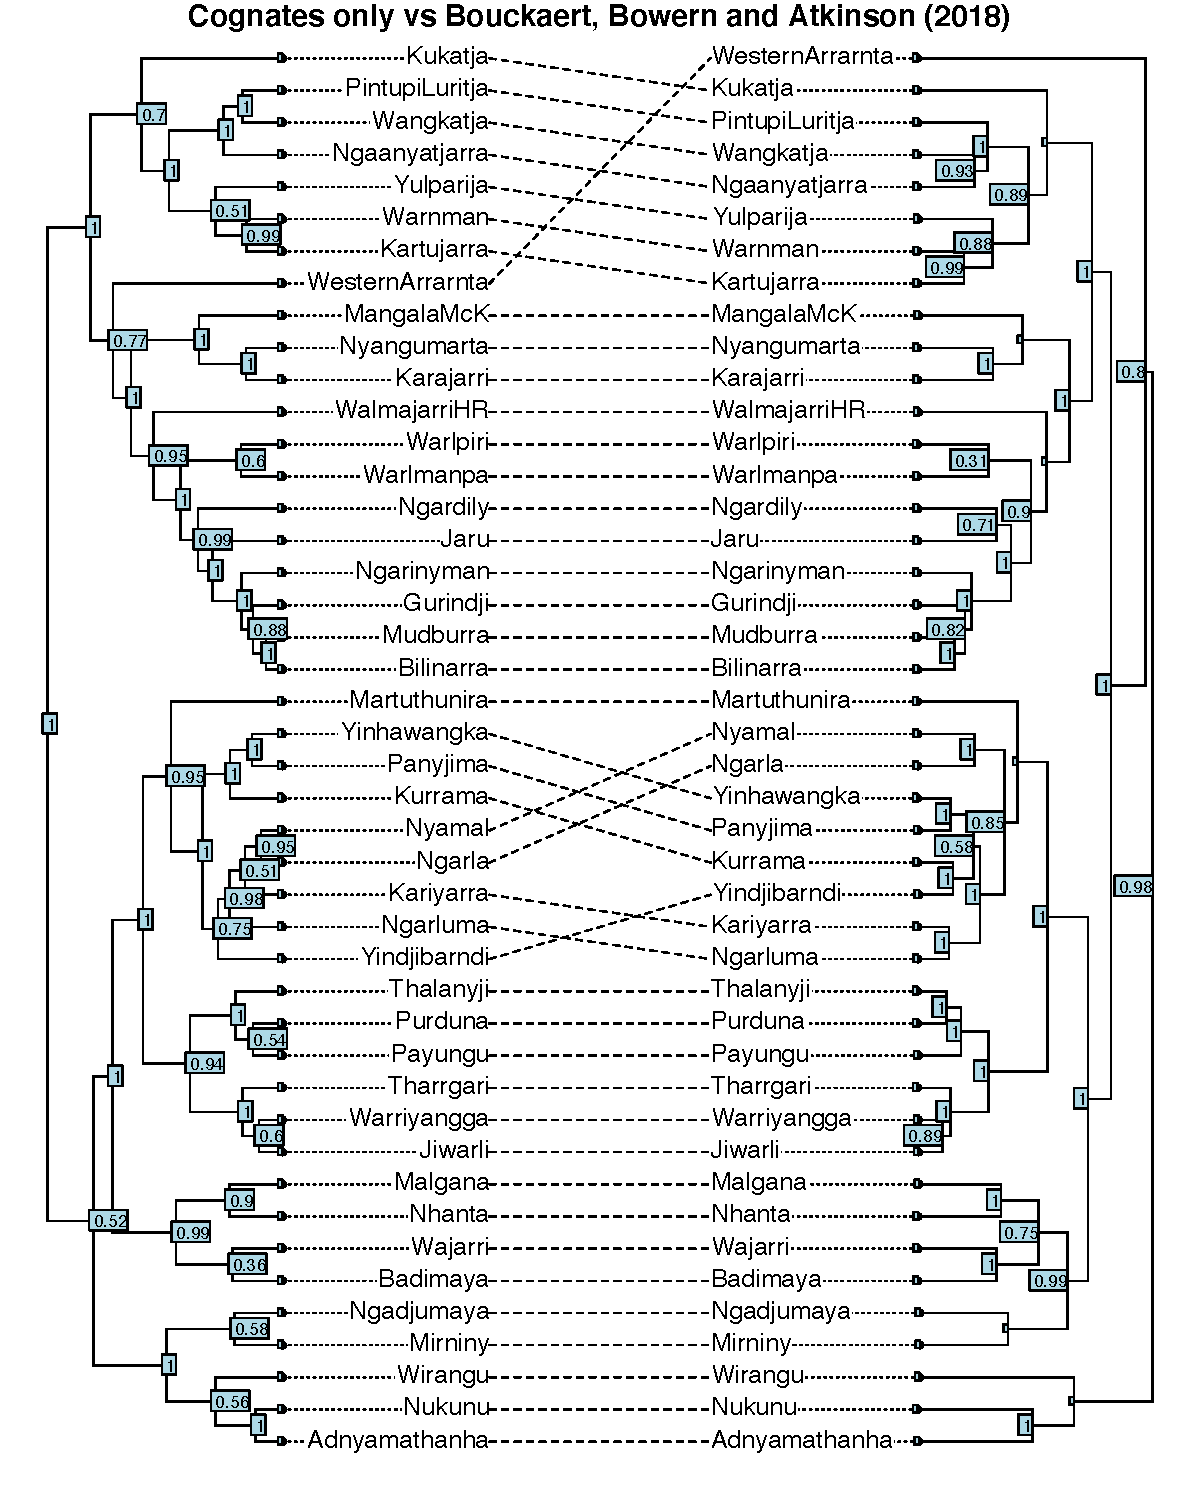
\includegraphics{fig/cogs_vs_bba2018.pdf}

\hypertarget{main-test-tree-inference-with-phonotactic-data}{%
\section{Main test: Tree inference with phonotactic data}\label{main-test-tree-inference-with-phonotactic-data}}

\hypertarget{data}{%
\subsection{Data}\label{data}}

There are three main sources of data for this experiment. One is cognate data from \textcite{bouckaert_origin_2018}, to which we apply an evolutionary model following \textcite{bouckaert_origin_2018}, as evaluated in Preliminary Test 2 (Section \ref{prelim-2}). There are two sets of phonotactic data, one binary and one continuous. Binary biphone data, which codes the presence or absence of biphones---sequences of two phonemes---in each language, is included with the best supported evolutionary model evaluated in Preliminary Test 1 (Section \ref{prelim-1}). Finally, we use a dataset of continuous phonotactic characters coding frequencies of transitions between natural sound classes. The data extraction process is detailed further as follows. Each consonant phoneme appearing in our wordlist data is binned into two natural classes, one for place of articulation and one for manner of articulation. Place classes are labial, dental, alveolar, retroflex, palatal and velar. Manner classes are obstruent, nasal, vibrant, lateral, glide, and rhotic glide. For the purposes of this experiment, we group all vowels into a single `vowel' class and also include word boundaries. The choice of place and manner natural classes is based on well-established principles of organisation among segments in Australian languages \autocites{dixon_languages_1980}{hamilton_phonetic_1996}{baker_word_2014}{round_segment_2021}{round_phonotactics_2021}. From each wordlist, we extract the frequency of a sound class \(x\) followed by a sound class \(y\), relativized over all instances of sound class \(x\). For use in BEAST, we logit-transform all the data to move from a 0--1 frequency interval to the real line. To include 0 and 1 frequency values in the logit-transformation, we follow a standard procedure of converting 0 values to \(\frac{min}{2}\), i.e.~half the smallest non-zero value, and converting 1 values to \(0.5 (1 + max)\), i.e.~half way between 1 and the maximum value less than 1. The evolutionary model applied to sound class transition frequency data in BEAST is a simple Brownian motion model which allows character values to wander up or down with equal possibility. We initially considered applying a single multivariate Brownian motion model to all continuous traits, however, the computational memory and time required by a multivariate Brownian motion model scales exponentially as the number of characters is increased. Instead, we fit a Brownian motion model to each character individually. This greatly increases the number of parameters in the overall model and potentially makes it less realistic, but it keeps the project computationally feasible. We return to this topic further in the discussion.

The choice of phonotactic data warrants brief further comment. We select sound class transition frequency data for a few reasons. One is that it partially, though not entirely, accounts for a lack of independence between biphone characters. This is because phonological rules, phonotactic restrictions and historical sound changes typically affect natural classes of phonemes rather than individual phonemes. This is not a perfect solution---sound classes themselves are independent from one another to varying degrees. A second reason is that \textcite{macklin-cordes_phylogenetic_2020} find a stronger degree of phylogenetic signal in sound class transition frequency data compared to transition frequencies between individual phonemes. A third reason is computational. A dataset of continuous characters equivalent in size to the binary biphone dataset would increase the computational time required to run BEAST by orders of magnitude, rendering the study impractical.

As mentioned in Section \ref{prelim-2}, we reduce the language sample to 44 western Pama-Nyungan languages. This was necessary to keep the computational demands of the experiment reasonable. We selected the western branch of Pama-Nyungan due to it being relatively well-attested in modern sources compared to those in, for example, the south-east of Australia where language documentation is more often reliant on archival sources due to the disproportionate impact of colonialism in this part of the continent.

We run BEAST on two phylogenetic models: a `linked' model, which contains a single tree likelihood term calculated using all cognate and phonotactic data, and a `seperate' model, which contains two tree likelihood terms, one calculated using cognate data only and the other using phonotactic data only (both binary and continuous). We run ten independent MCMC chains of 100 million iterations on each model, inspect and combine the results, estimate marginal likelihoods for each of the `linked' and `separate' models and generate three maximum clade credibility trees (one for the `linked' model, and one each for the cognate-only and phonotactics-only elements of the `separate' model).

\hypertarget{main-results}{%
\subsection{Results}\label{main-results}}

One first observation is that, although the MCMC process in BEAST tends to converge over 100 million states, it can also get stuck in local optima within the probability space. When this became clear, we increased the number of independent chains from an initial four to ten. Inspecting the joint probability traces for each of the linked model's ten runs, we find one clearly preferred area of the state space. We remove the one clear outlier run stuck in a local optimum above the state space. Two additional runs are removed since, although they overlap considerably with the others, they too seem to represent a distinct local optimum in the state space. One additional run was removed as it had unusually low ESS values. After removing 15\% initial burn-in and combining the remaining chains, we are left with a combined 340-million-state analysis. The combined log marginal likelihood estimates are 564,009 (estimated via path sampling) and 988,203 (estimated via stepping stone sampling). Unfortunately, it is unclear whether or not these log MLE figures are meaningful. Log MLEs for each individual chain vary between 459,380 and 672,466 which is much more variation than we would expect, given that a difference of 20 is generally considered significant. Given that all chains represent the same data and model and converge in approximately the same space, we would expect their log MLEs to be roughly equivalent. We discuss this further below.

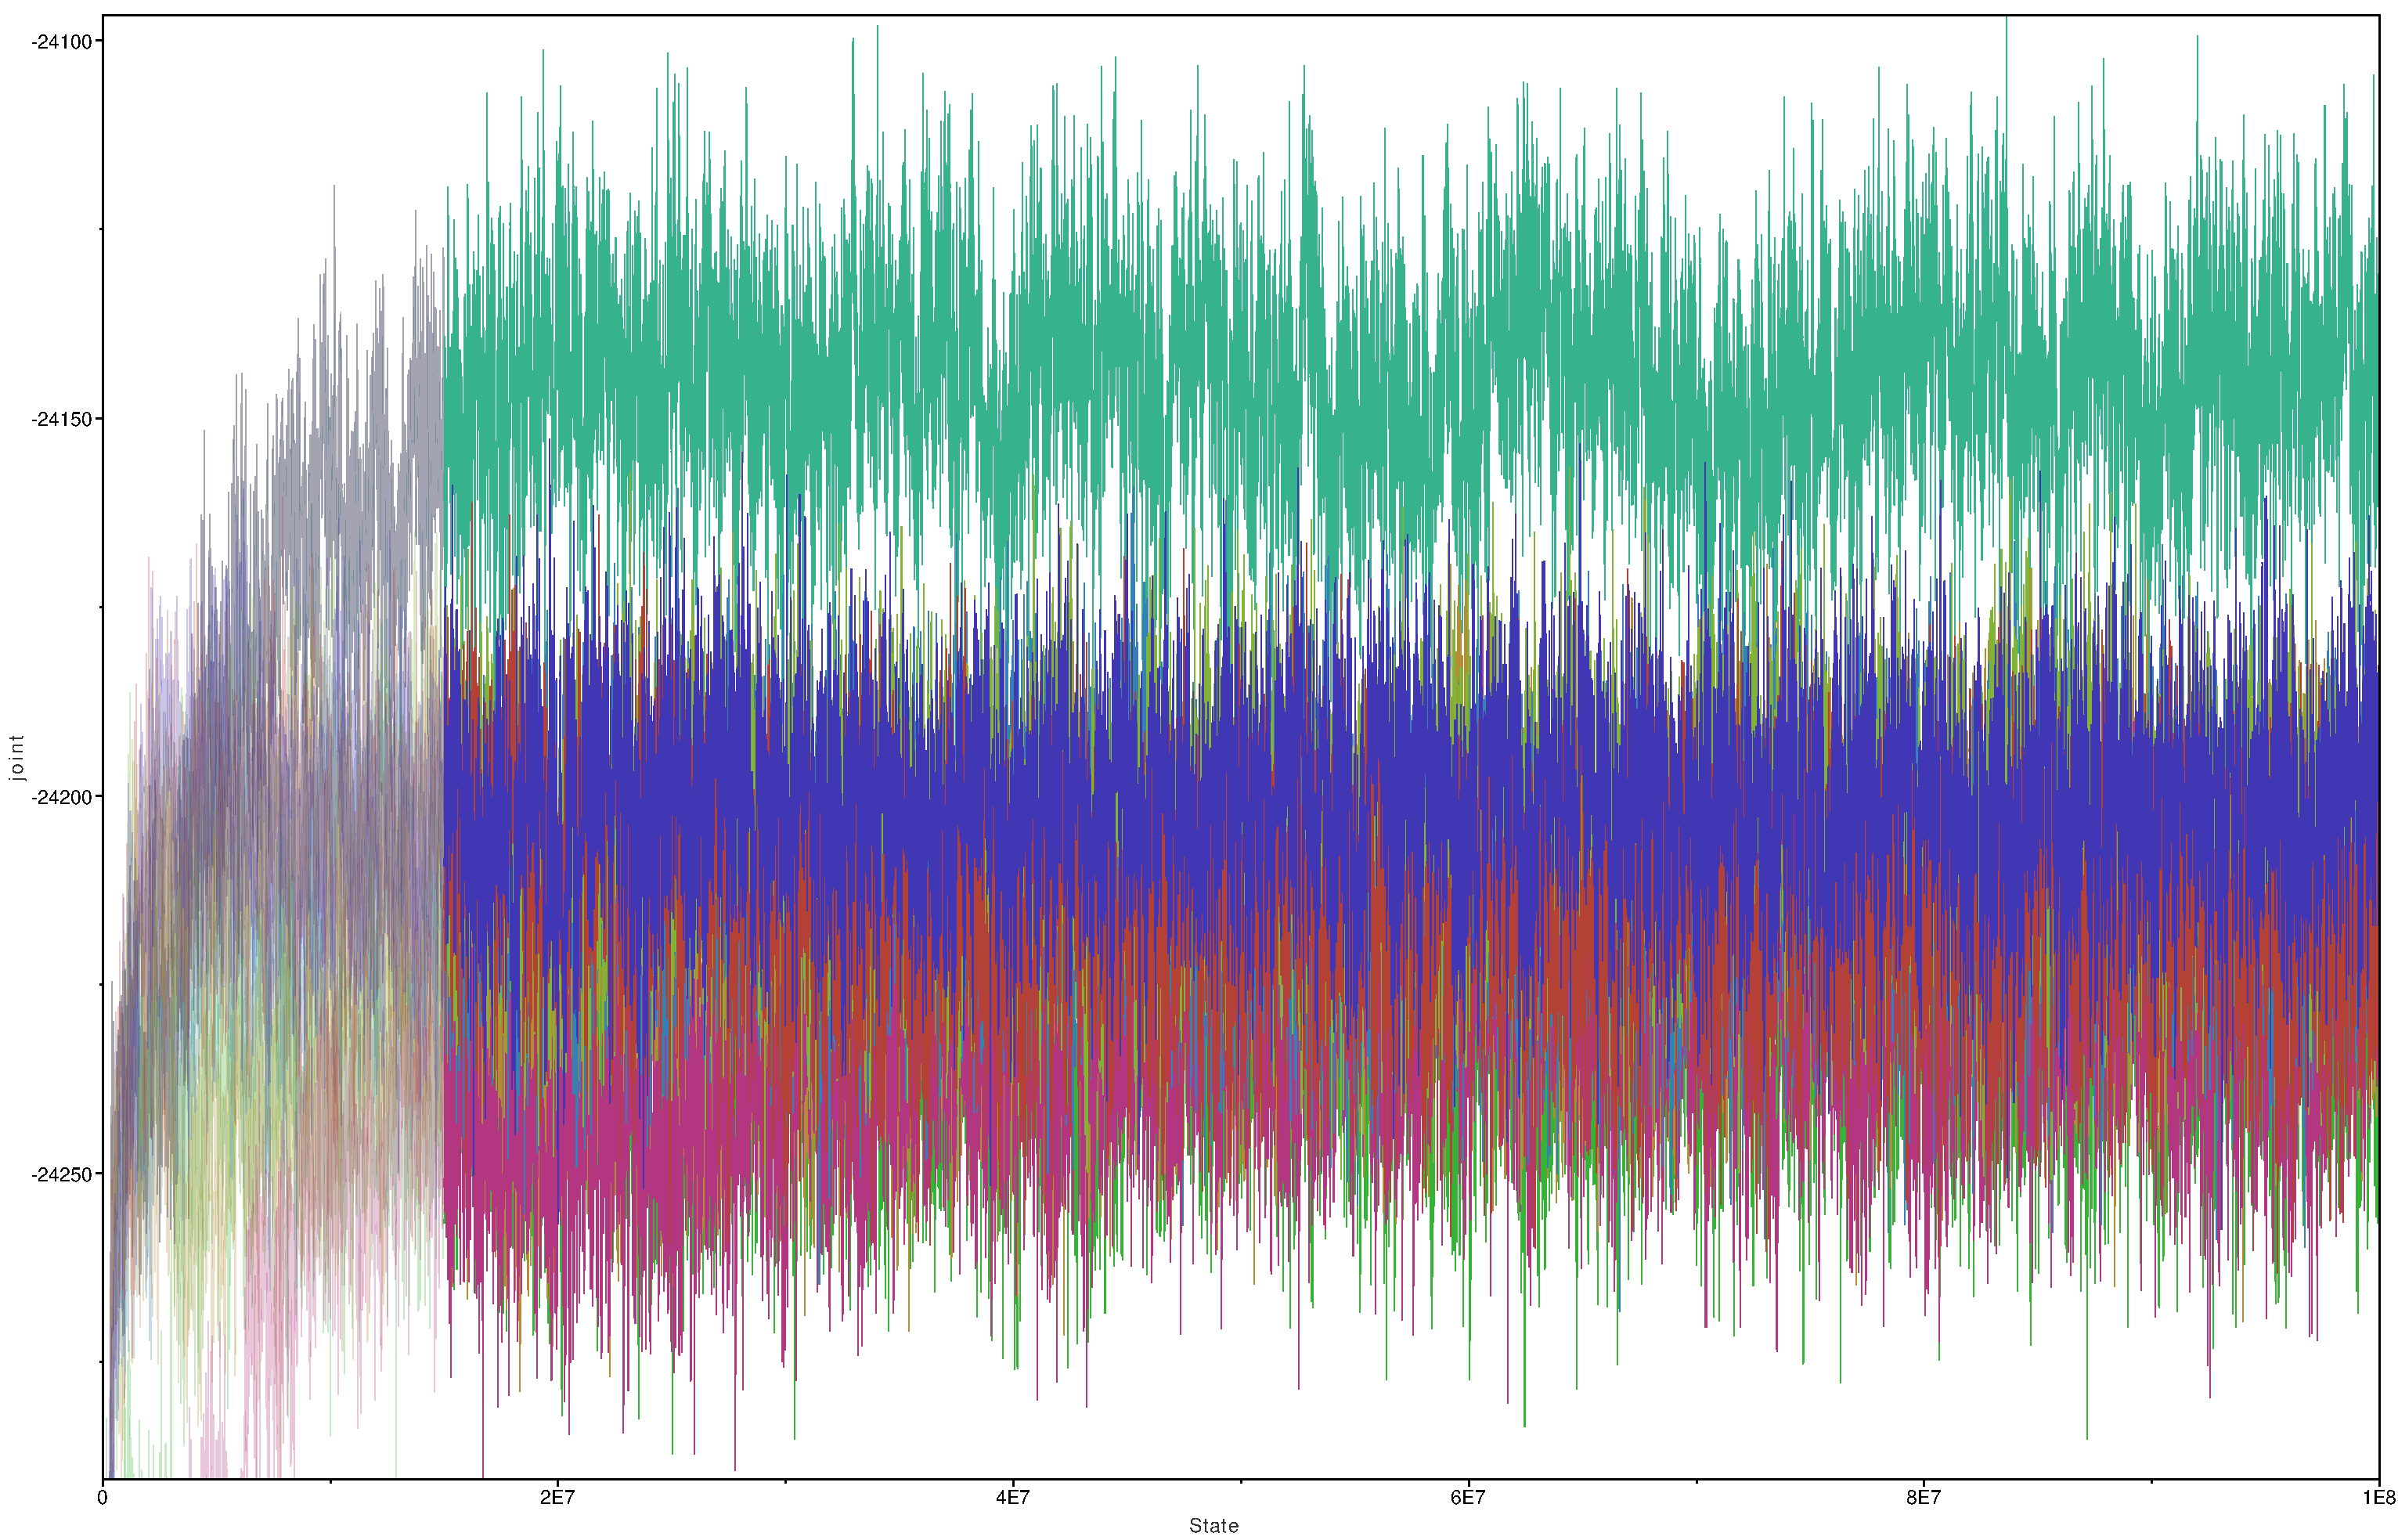
\includegraphics{fig/joint_trace_ch1-10.pdf}
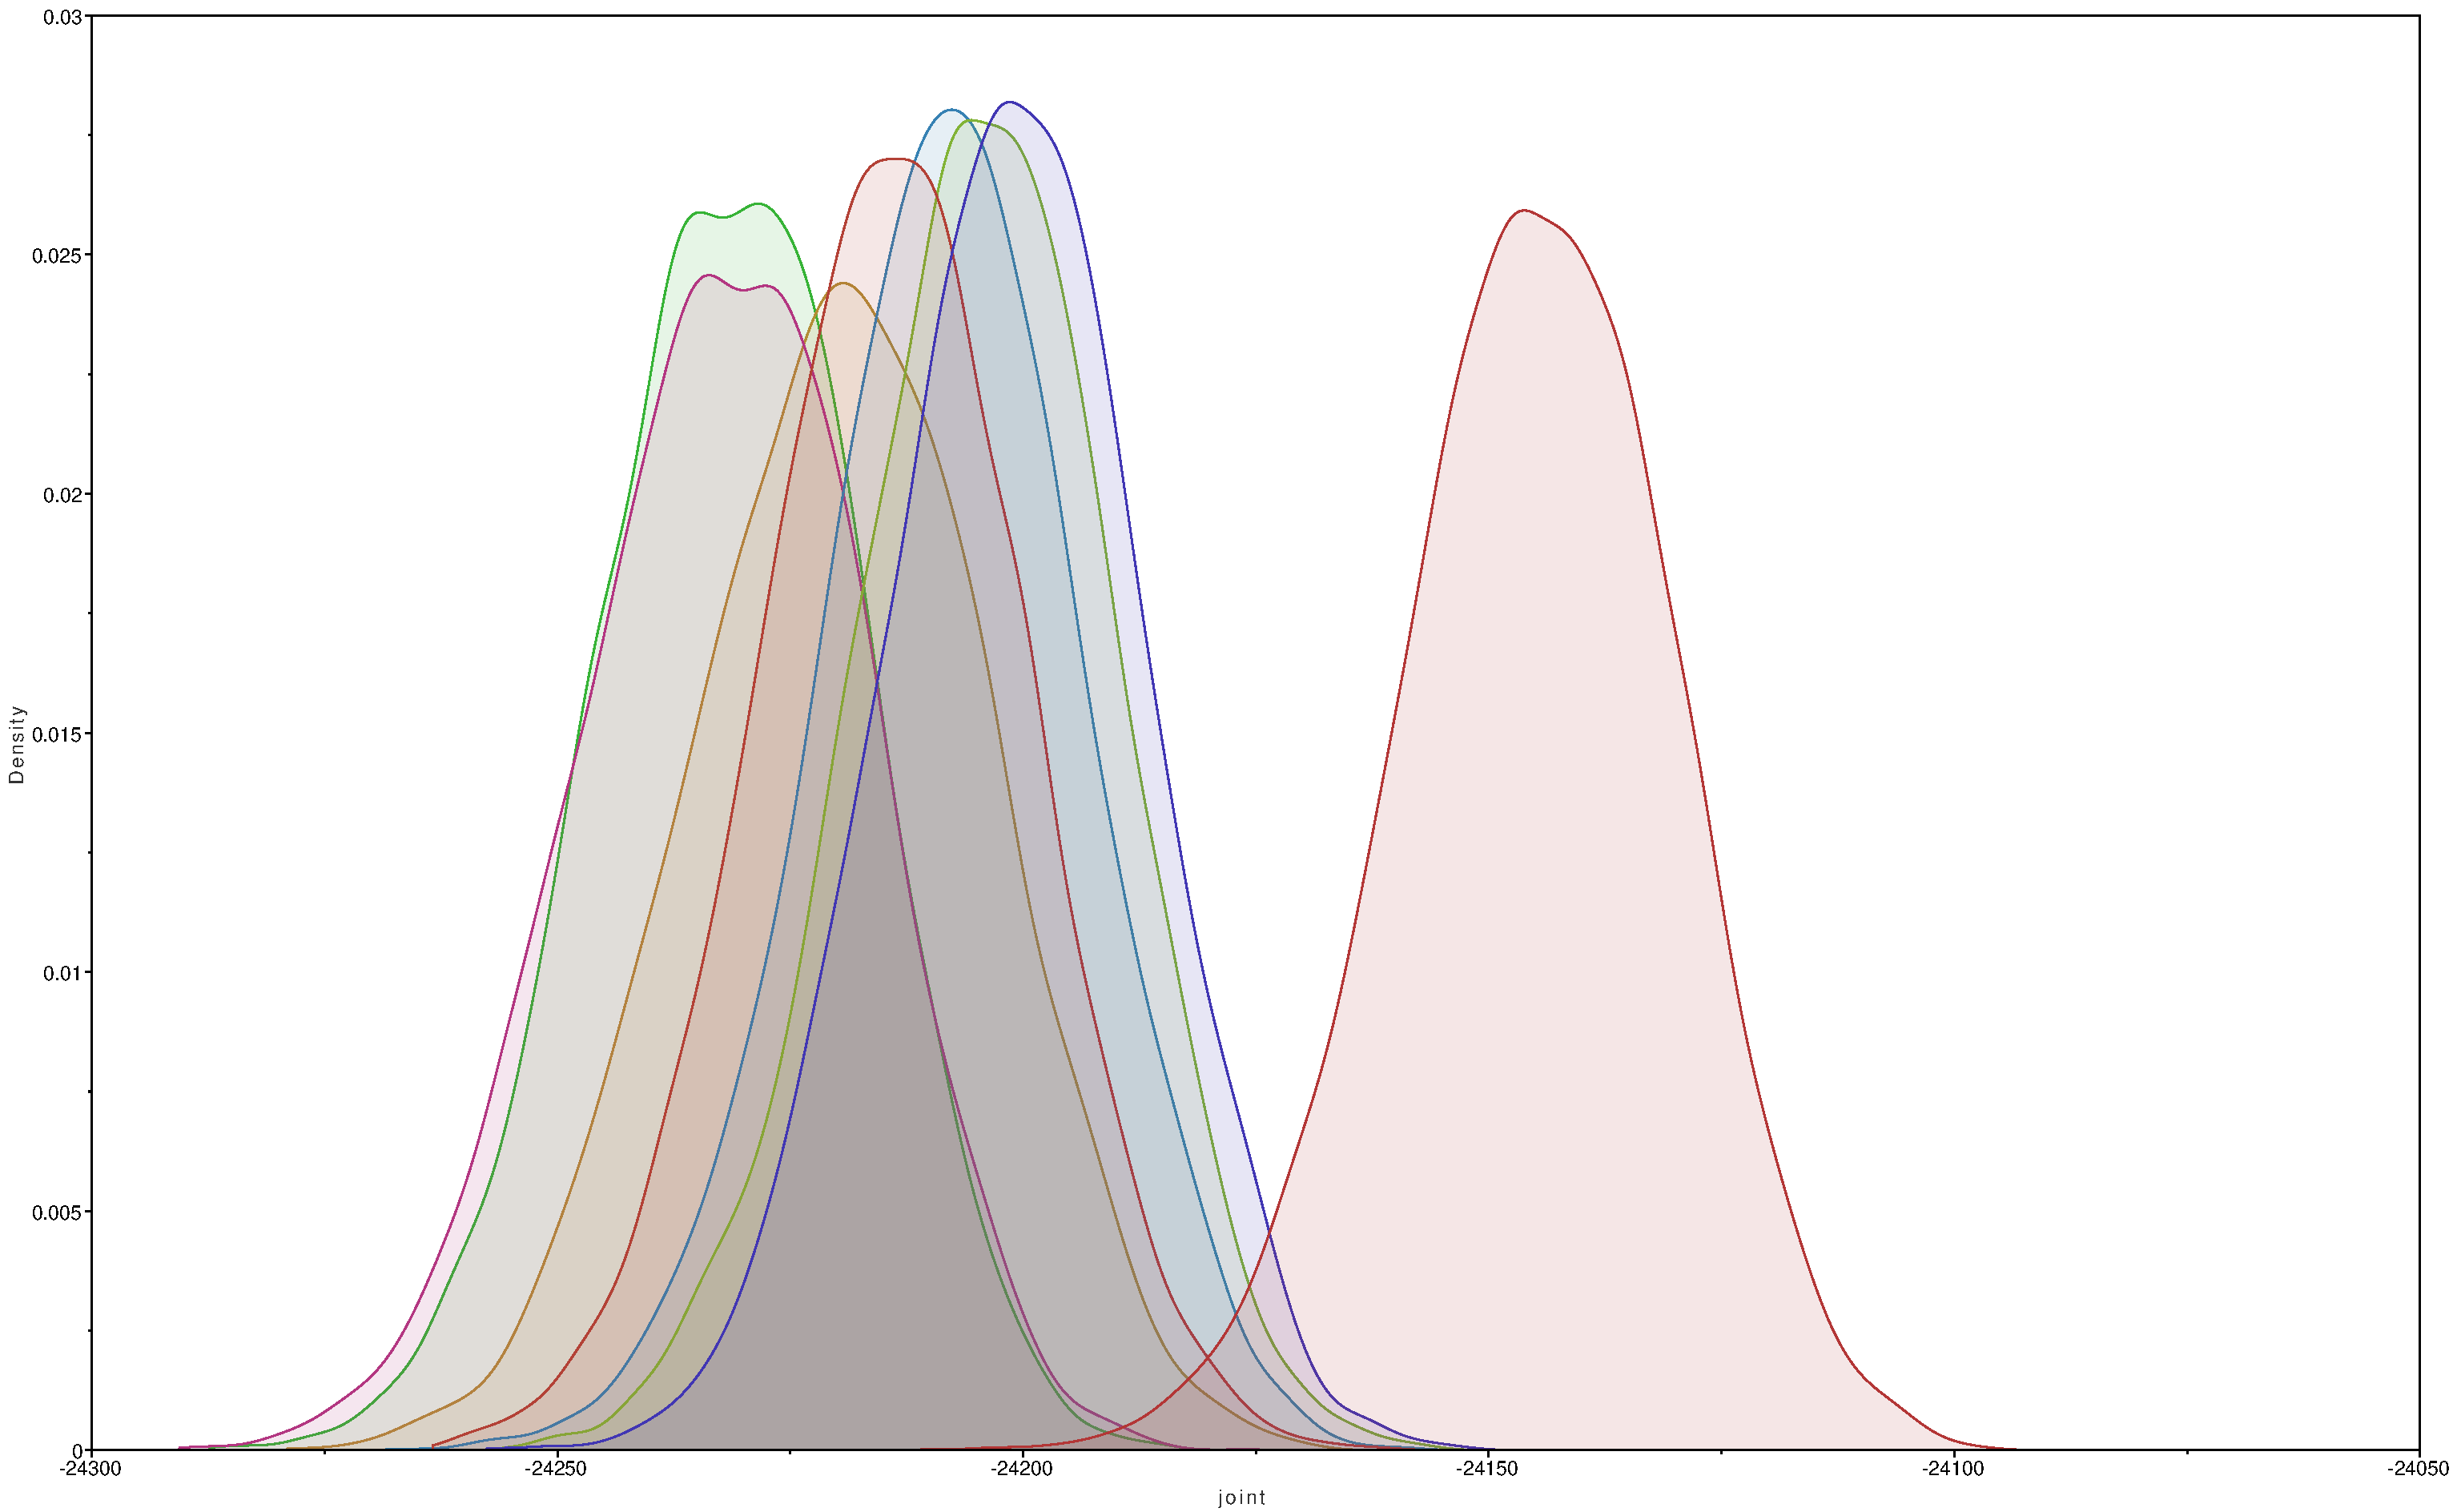
\includegraphics{fig/joint_trace_dens_1-2_5-10.pdf}

The separate model, in which two trees are sampled at each step, one inferred using only cognate data and one inferred using only phonotactic data, similiarly shows a tendency to get stuck in local optima and converge in different parts of the state space from one run to another. One chain was discarded for failing to reach a stable convergence. Two others were discarded for unsuitably low ESS values. This leaves one chain with a stable convergence after 10\% burn-in and ESS values all 150 or greater, including an ESS of 508 for joint probability. The log MLEs for the separate model are 530,001 (estimated via path sampling) and 567,677 (estimated via stepping stone sampling). The linked and separate models can be compared using Bayes factors, as per Equation \eqref{eq:bf}.

\begin{equation}
BF = log(MLE_{linked}) - log(MLE_{separate})
\label{eq:bf}
\end{equation}

The sign of the Bayes factor indicates which model is preferred. In this case, if we use the MLEs estimated via path sampling, the Bayes factor is \(-70,621\), suggesting the separate model fits best. On the other hand, the Bayes factor for MLEs estimated via stepping stone sampling is \(420,526\), suggesting the linked model fits best. This reenforces the impression that MLEs are not being estimated accurately.

To compare the phylogeny inferred using the linked model, which includes phonotactics, to the phylogeny inferred using only cognate data in the previous section, we examine maximum clade credibility trees estimated from each. The cophylogenetic plot is given in Figure \ref{cogs-vs-linked-all}.

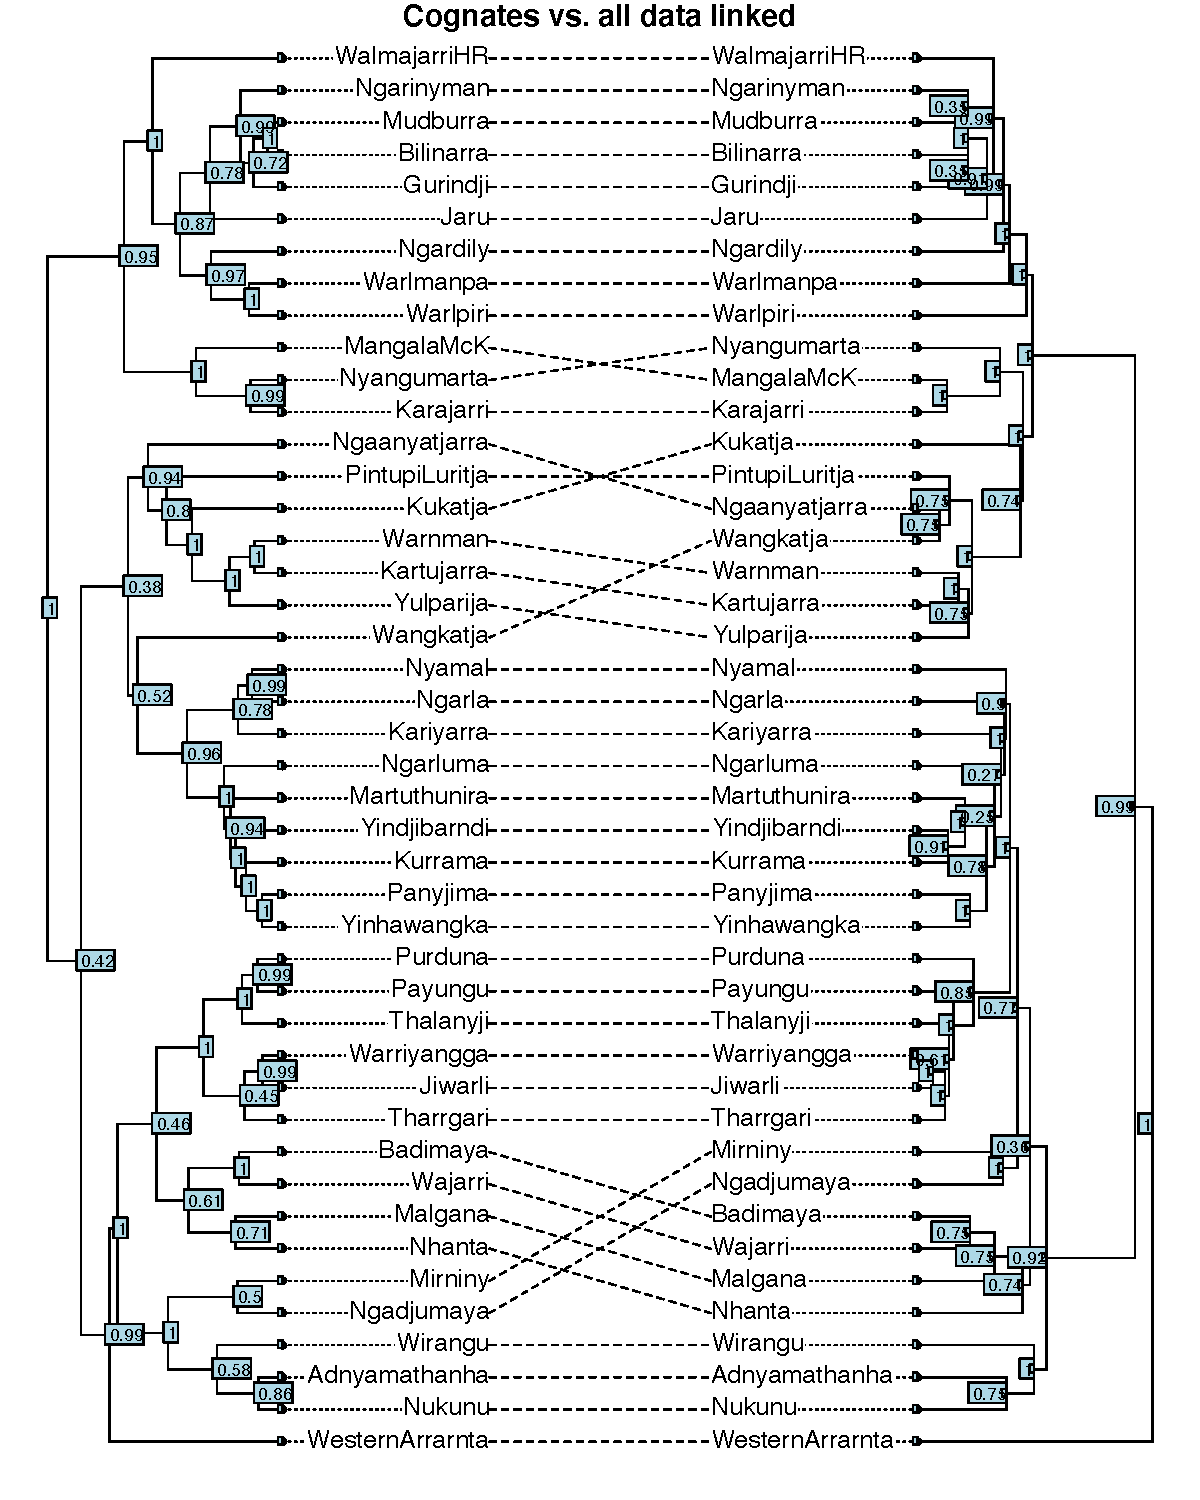
\includegraphics{fig/cogs_vs_linked_all.pdf}

Likely need to run for much longer and more times, with operators altered to allow bigger jumps in order to escape optima.

\hypertarget{main-test-follow-up-removing-binary-biphone-data}{%
\section{Main test follow-up: Removing binary biphone data}\label{main-test-follow-up-removing-binary-biphone-data}}

\hypertarget{pn-tree-discussion}{%
\section{Discussion}\label{pn-tree-discussion}}

Discussion in biology regarding combination of morphological and genomic datasets. ``Simultaneous'' approach where both morphological and genomic data are used jointly to infer the tree versus ``scaffolding'' approach where only genomic data is used to infer tree topology, then morphological data is used to assess e.g.~dating (using fossil record) while being constrained to genomic tree topology \autocite{lee_morphological_2015}. Must be aware of the potential circularity of tracing the evolution of characters on a phylogeny which was itself partly based on those characters \autocite{de_queiroz_including_1996}.

Limitations:

\begin{itemize}
\tightlist
\item
  Logical dependencies between variables (because of sound changes, phonotactic restrictions affecting natural classes)
\item
  Logical dependencies between binary/continuous partitions (non-gap in freq data = 1 in binary data. 0 in binary data = gap in freq data)
\item
  Didn't account for sound change
\item
  Limitations of Brownian motion model
\end{itemize}

If we get a negative result (no significant difference between trees inferred with/without phonotactic data partition) then I would speculate that it's probably got a lot to do with the inability of our Brownian motion evolutionary model to capture the effects of sound change, which would manifest as sudden jumps in frequencies.

If we get a positive result, then we would advocate for the use of phonotactic data in combination with other sources of evidence, such as cognate data, to infer linguistic phylogenies.

\begin{itemize}
\tightlist
\item
  Could be used to help resolve phylogenetic conflicts in places where there is more phylogenetic uncertainty. Could be used to help with dating and branch lengths in places where otherwise the topology is quite well understood.
\item
  Could help in under-resourced places that don't have as much lexical data. Studies of Pama-Nyungan phylogeny have benefitted from reasonably extensive cognate coding over nearly 300 meaning classes, but a lot of places will be limited to the scale of Swadesh lists or even less. (The opposite is true in biology, where morphological datasets make up ever shrinking proportion of total combined dataset when combined with genomic datasets that keep getting bigger)
\item
  Could be used for quick and dirty tree inference where some phylogenetic information is required/better than nothing (for example, using phylogenetic comparative methods) but doesn't necessarily have to be perfect. e.g.~could combine with very small lexical datasets/automatic cognate identification. Perhaps could be combined with, e.g.~glottolog classifications to get something consistent with glottolog tree but fully resolved.
\end{itemize}

\newpage

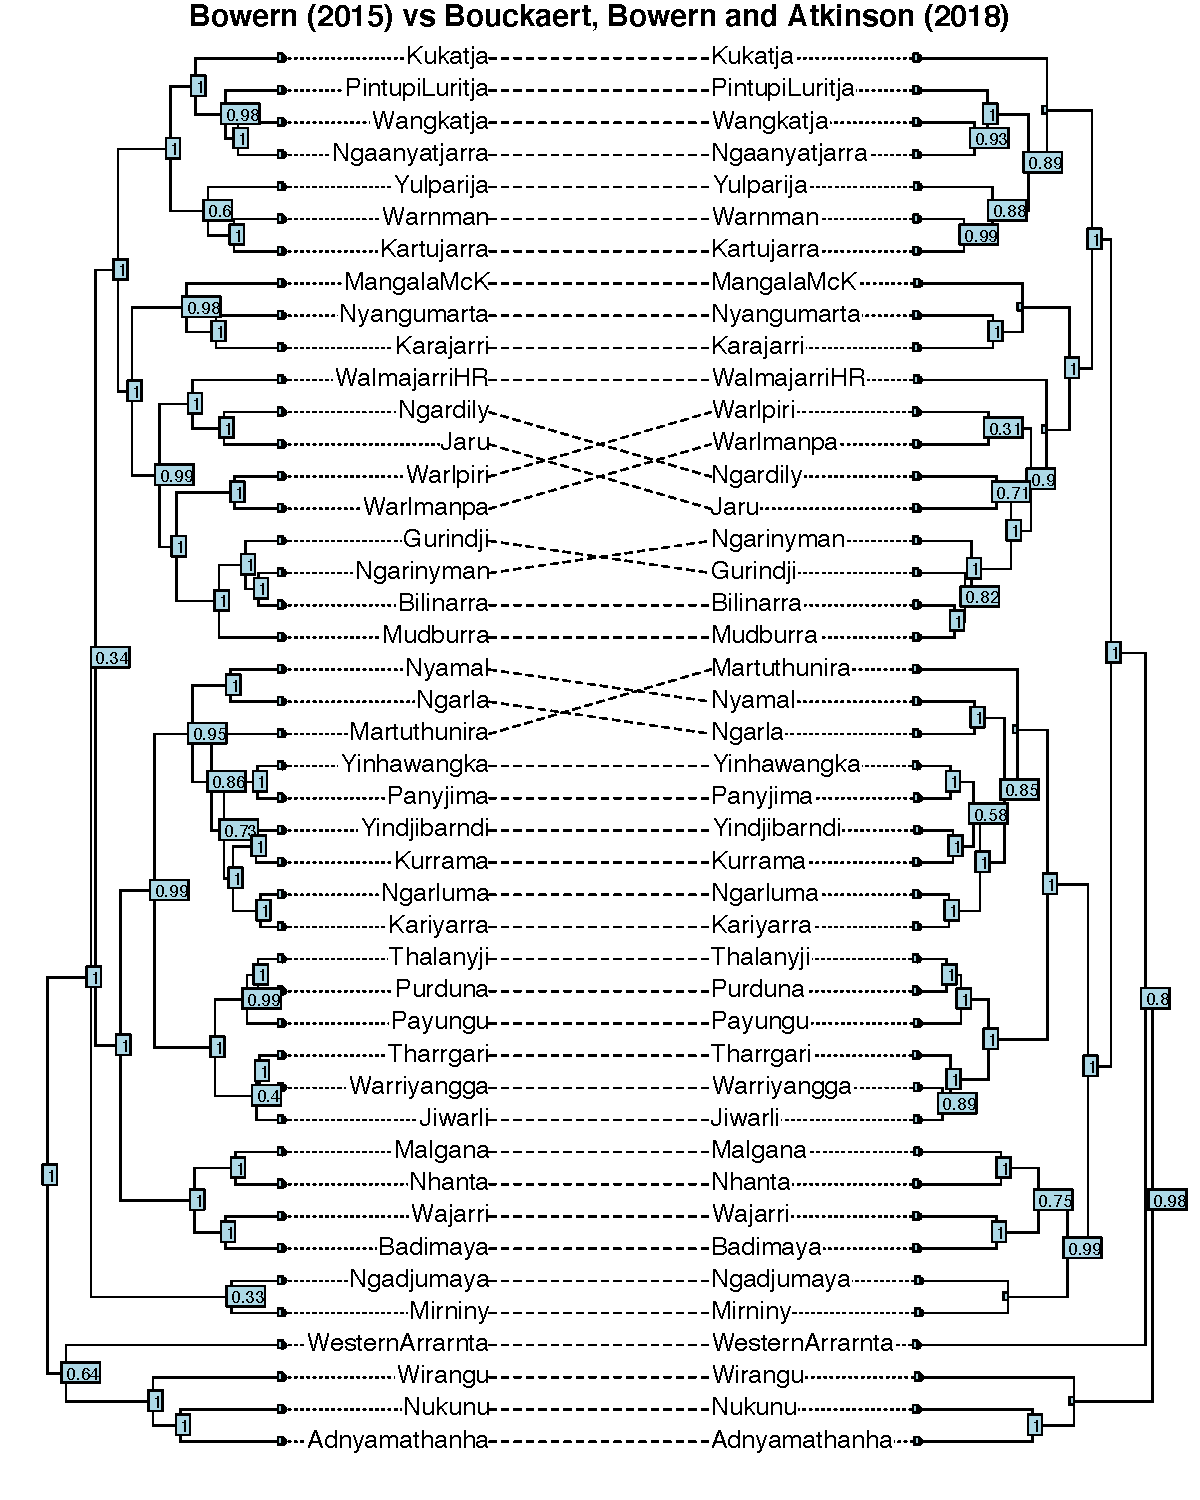
\includegraphics{fig/cb2015_vs_bba2018.pdf}

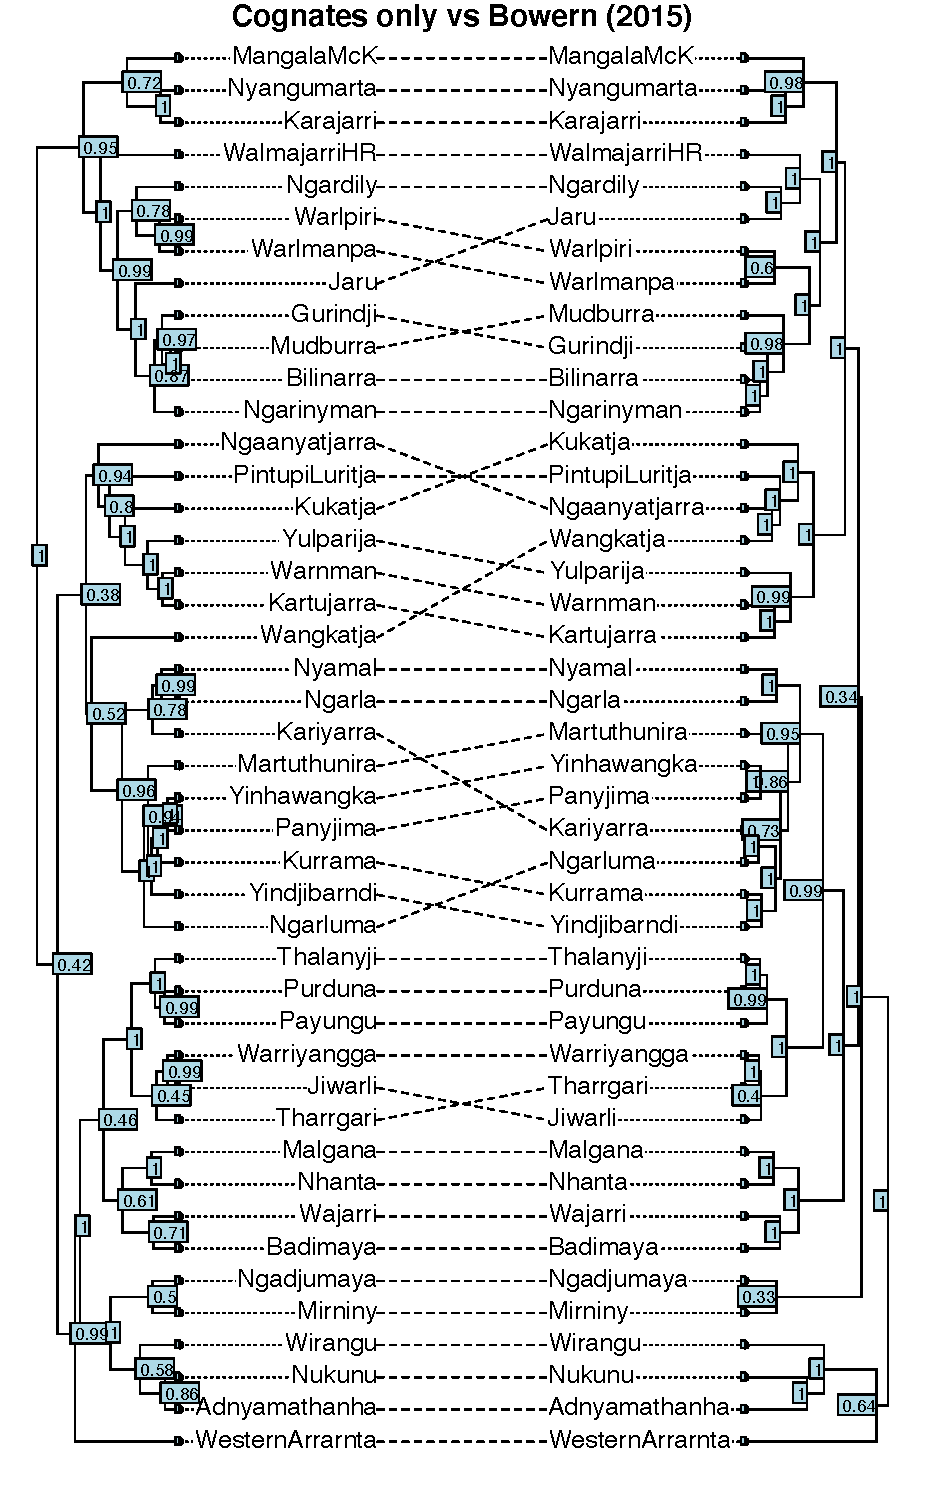
\includegraphics{fig/cogs_vs_cb2015.pdf}

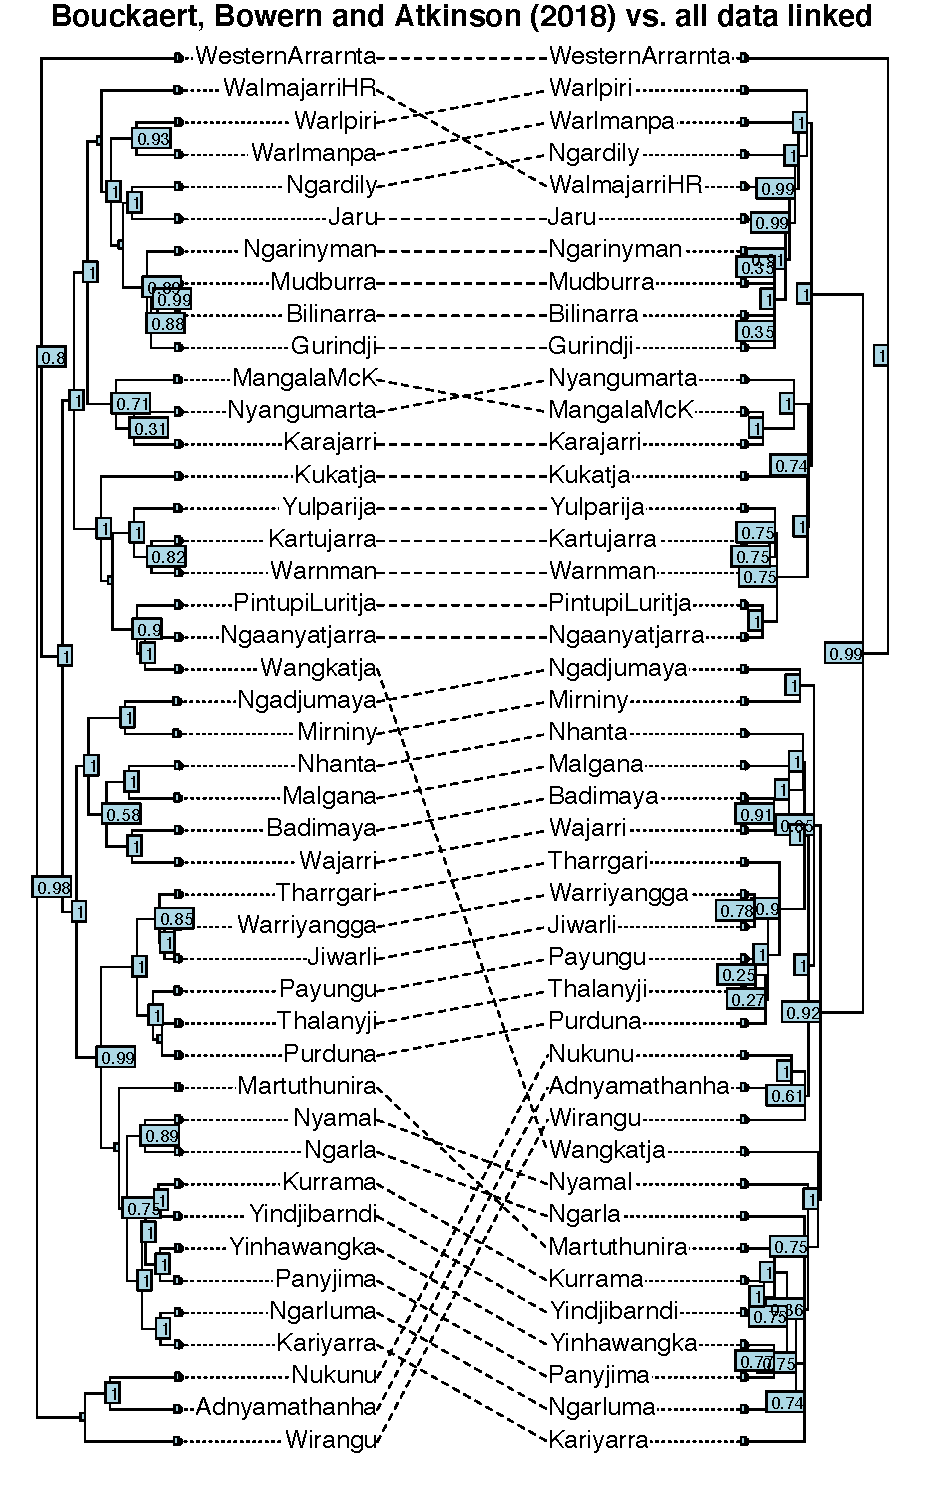
\includegraphics{fig/bba2018_vs_linked_all.pdf}

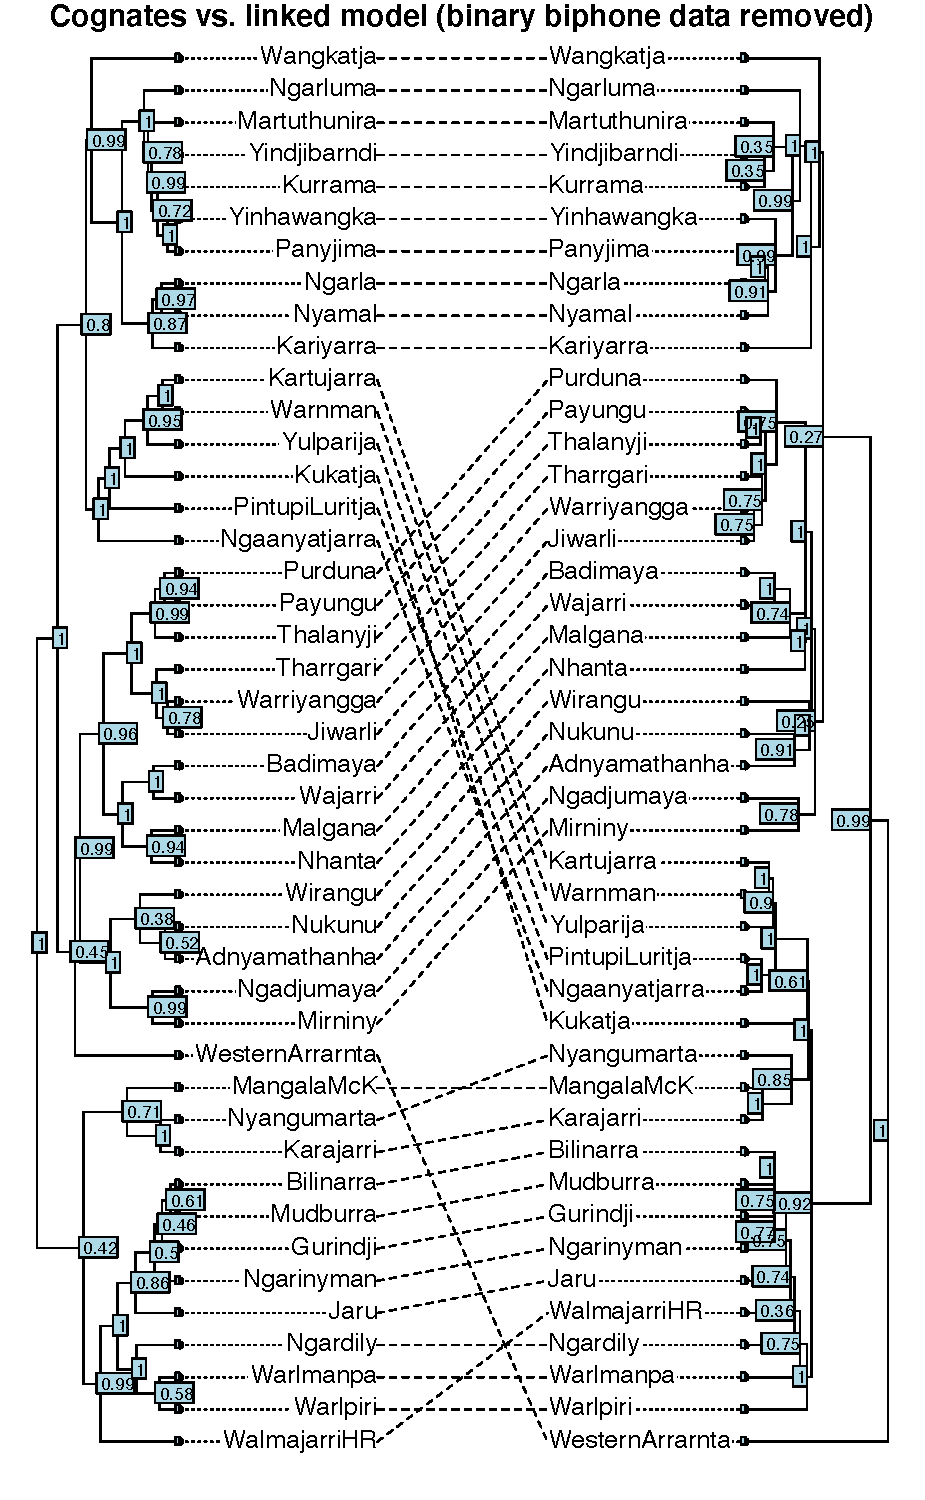
\includegraphics{fig/cogs_vs_linked.pdf}

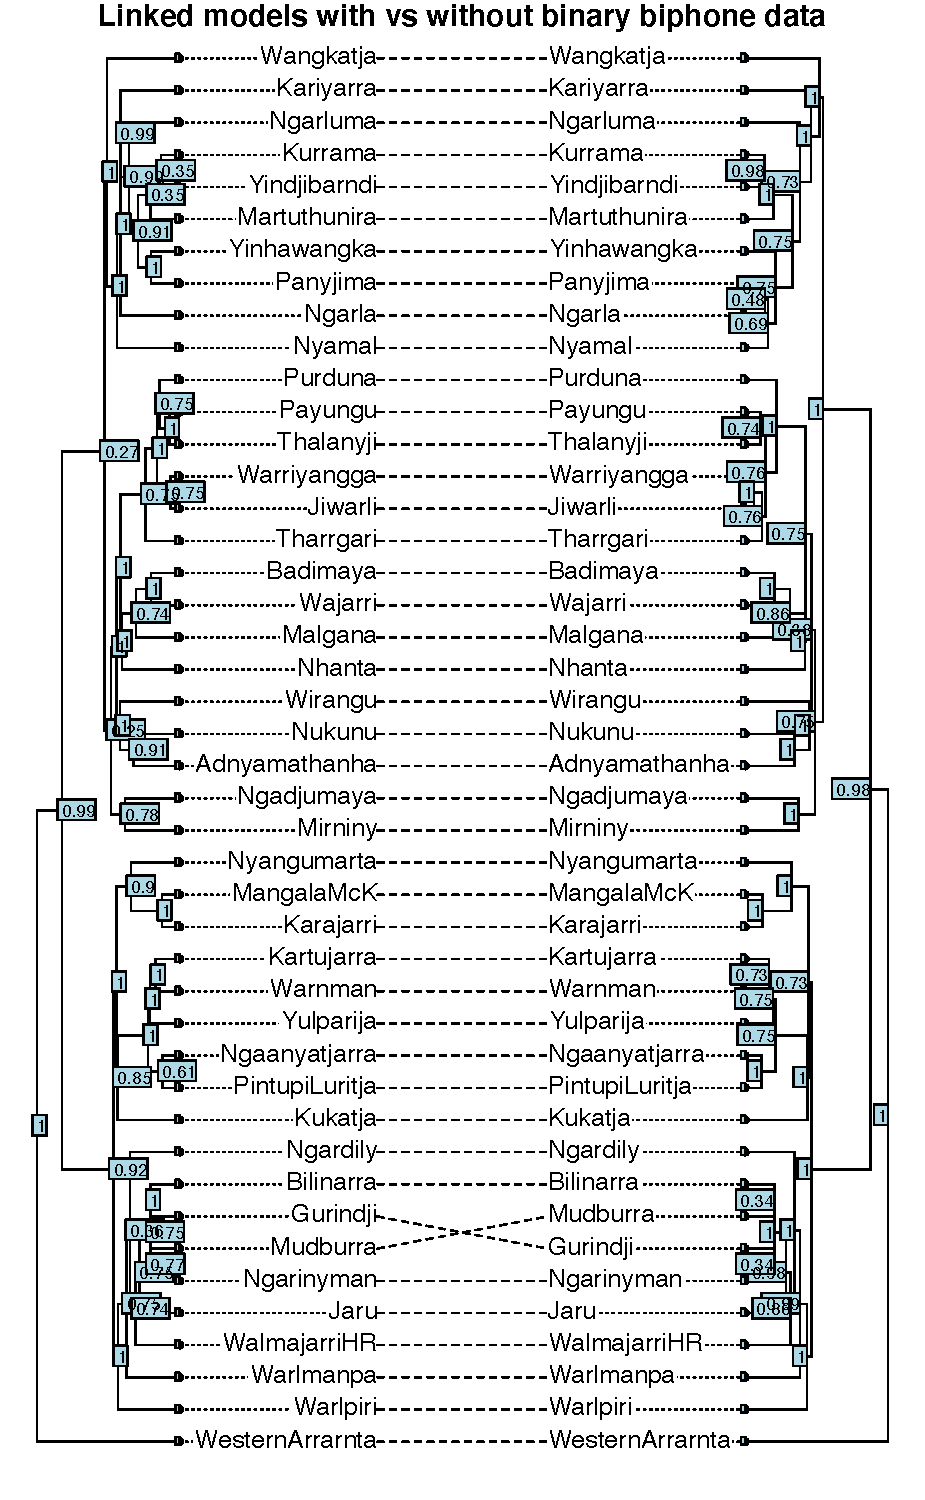
\includegraphics{fig/linked_all_vs_linked.pdf}

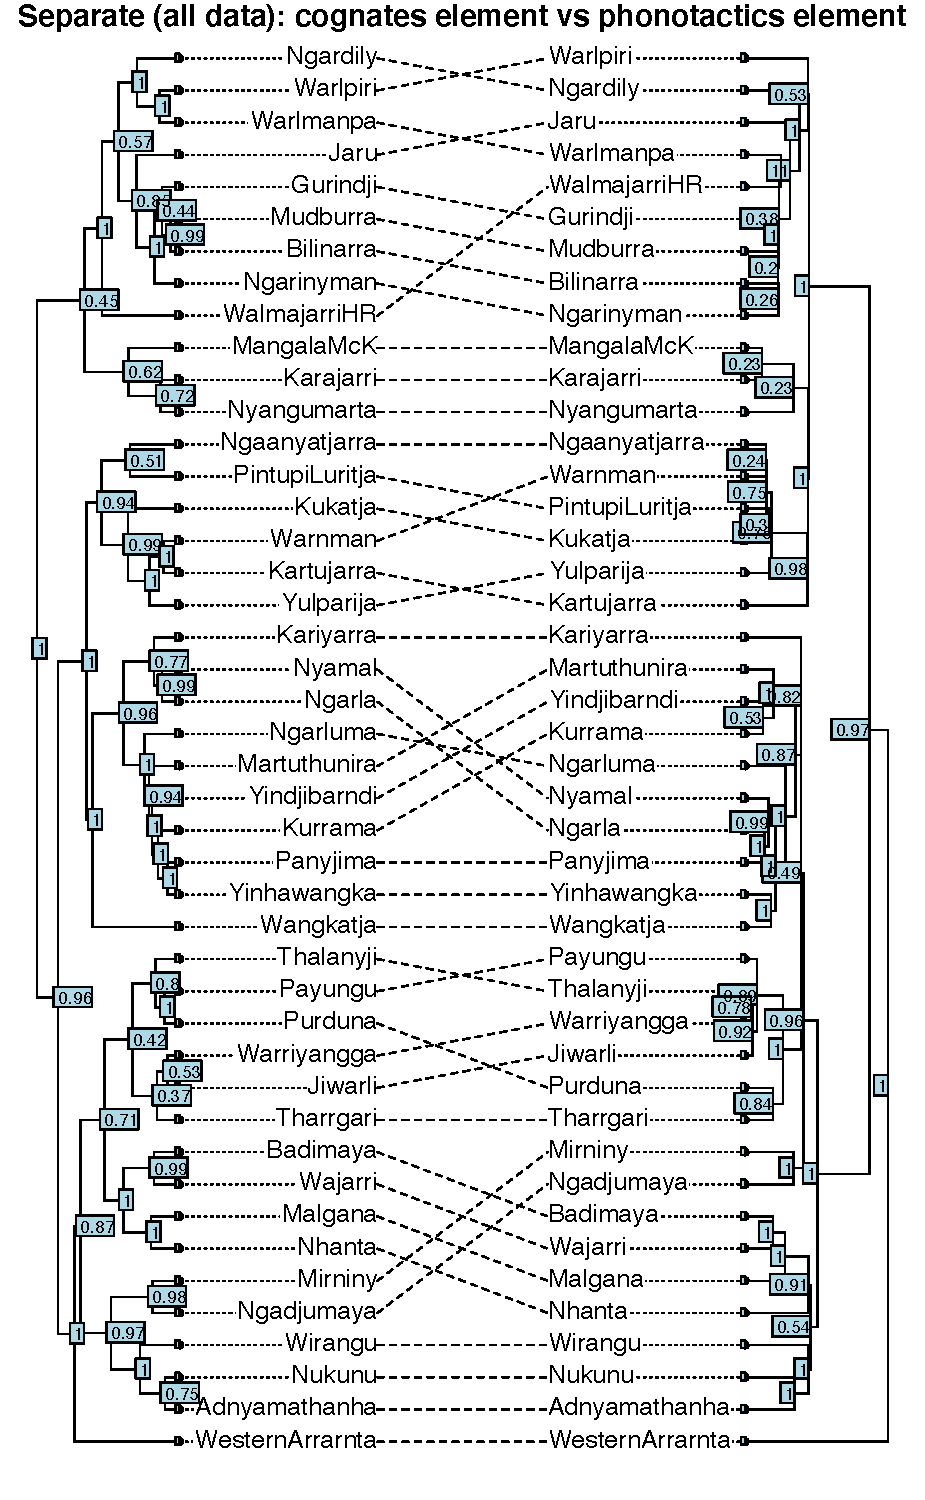
\includegraphics{fig/separate_cogs_vs_phonotactics_alldata.pdf}

\hypertarget{conclusion}{%
\section{Conclusion}\label{conclusion}}

\printbibliography

\end{document}
